\documentclass[twoside]{book}

% Packages required by doxygen
\usepackage{fixltx2e}
\usepackage{calc}
\usepackage{doxygen}
\usepackage[export]{adjustbox} % also loads graphicx
\usepackage{graphicx}
\usepackage[utf8]{inputenc}
\usepackage{makeidx}
\usepackage{multicol}
\usepackage{multirow}
\PassOptionsToPackage{warn}{textcomp}
\usepackage{textcomp}
\usepackage[nointegrals]{wasysym}
\usepackage[table]{xcolor}

% Font selection
\usepackage[T1]{fontenc}
\usepackage[scaled=.90]{helvet}
\usepackage{courier}
\usepackage{amssymb}
\usepackage{sectsty}
\renewcommand{\familydefault}{\sfdefault}
\allsectionsfont{%
  \fontseries{bc}\selectfont%
  \color{darkgray}%
}
\renewcommand{\DoxyLabelFont}{%
  \fontseries{bc}\selectfont%
  \color{darkgray}%
}
\newcommand{\+}{\discretionary{\mbox{\scriptsize$\hookleftarrow$}}{}{}}

% Page & text layout
\usepackage{geometry}
\geometry{%
  a4paper,%
  top=2.5cm,%
  bottom=2.5cm,%
  left=2.5cm,%
  right=2.5cm%
}
\tolerance=750
\hfuzz=15pt
\hbadness=750
\setlength{\emergencystretch}{15pt}
\setlength{\parindent}{0cm}
\setlength{\parskip}{3ex plus 2ex minus 2ex}
\makeatletter
\renewcommand{\paragraph}{%
  \@startsection{paragraph}{4}{0ex}{-1.0ex}{1.0ex}{%
    \normalfont\normalsize\bfseries\SS@parafont%
  }%
}
\renewcommand{\subparagraph}{%
  \@startsection{subparagraph}{5}{0ex}{-1.0ex}{1.0ex}{%
    \normalfont\normalsize\bfseries\SS@subparafont%
  }%
}
\makeatother

% Headers & footers
\usepackage{fancyhdr}
\pagestyle{fancyplain}
\fancyhead[LE]{\fancyplain{}{\bfseries\thepage}}
\fancyhead[CE]{\fancyplain{}{}}
\fancyhead[RE]{\fancyplain{}{\bfseries\leftmark}}
\fancyhead[LO]{\fancyplain{}{\bfseries\rightmark}}
\fancyhead[CO]{\fancyplain{}{}}
\fancyhead[RO]{\fancyplain{}{\bfseries\thepage}}
\fancyfoot[LE]{\fancyplain{}{}}
\fancyfoot[CE]{\fancyplain{}{}}
\fancyfoot[RE]{\fancyplain{}{\bfseries\scriptsize Generated by Doxygen }}
\fancyfoot[LO]{\fancyplain{}{\bfseries\scriptsize Generated by Doxygen }}
\fancyfoot[CO]{\fancyplain{}{}}
\fancyfoot[RO]{\fancyplain{}{}}
\renewcommand{\footrulewidth}{0.4pt}
\renewcommand{\chaptermark}[1]{%
  \markboth{#1}{}%
}
\renewcommand{\sectionmark}[1]{%
  \markright{\thesection\ #1}%
}

% Indices & bibliography
\usepackage{natbib}
\usepackage[titles]{tocloft}
\setcounter{tocdepth}{3}
\setcounter{secnumdepth}{5}
\makeindex

% Hyperlinks (required, but should be loaded last)
\usepackage{ifpdf}
\ifpdf
  \usepackage[pdftex,pagebackref=true]{hyperref}
\else
  \usepackage[ps2pdf,pagebackref=true]{hyperref}
\fi
\hypersetup{%
  colorlinks=true,%
  linkcolor=blue,%
  citecolor=blue,%
  unicode%
}

% Custom commands
\newcommand{\clearemptydoublepage}{%
  \newpage{\pagestyle{empty}\cleardoublepage}%
}

\usepackage{caption}
\captionsetup{labelsep=space,justification=centering,font={bf},singlelinecheck=off,skip=4pt,position=top}

%===== C O N T E N T S =====

\begin{document}

% Titlepage & ToC
\hypersetup{pageanchor=false,
             bookmarksnumbered=true,
             pdfencoding=unicode
            }
\pagenumbering{alph}
\begin{titlepage}
\vspace*{7cm}
\begin{center}%
{\Large arduino\+\_\+\+D\+M\+X\+Pro \\[1ex]\large 09e4e24 }\\
\vspace*{1cm}
{\large Generated by Doxygen 1.8.13}\\
\end{center}
\end{titlepage}
\clearemptydoublepage
\pagenumbering{roman}
\tableofcontents
\clearemptydoublepage
\pagenumbering{arabic}
\hypersetup{pageanchor=true}

%--- Begin generated contents ---
\chapter{arduino\+\_\+\+D\+M\+X\+Pro}
\label{index}\hypertarget{index}{}\input{index}
\chapter{Namespace Index}
\section{Namespace List}
Here is a list of all namespaces with brief descriptions\+:\begin{DoxyCompactList}
\item\contentsline{section}{\hyperlink{namespaceDMXPro}{D\+M\+X\+Pro} }{\pageref{namespaceDMXPro}}{}
\end{DoxyCompactList}

\chapter{Class Index}
\section{Class List}
Here are the classes, structs, unions and interfaces with brief descriptions\+:\begin{DoxyCompactList}
\item\contentsline{section}{\hyperlink{classDMXPro_1_1Processor}{D\+M\+X\+Pro\+::\+Processor$<$ ser\+\_\+typ $>$} }{\pageref{classDMXPro_1_1Processor}}{}
\item\contentsline{section}{\hyperlink{structDMXPro_1_1widget__parameters__non__user__defined}{D\+M\+X\+Pro\+::widget\+\_\+parameters\+\_\+non\+\_\+user\+\_\+defined} \\*Structure representing widget parameters that are not defined arbitrarily }{\pageref{structDMXPro_1_1widget__parameters__non__user__defined}}{}
\end{DoxyCompactList}

\chapter{File Index}
\section{File List}
Here is a list of all files with brief descriptions\+:\begin{DoxyCompactList}
\item\contentsline{section}{src/\hyperlink{arduino__DMXPro_8h}{arduino\+\_\+\+D\+M\+X\+Pro.\+h} \\*Header file for the arduino D\+MX Pro Widget Emulation Library }{\pageref{arduino__DMXPro_8h}}{}
\end{DoxyCompactList}

\chapter{Namespace Documentation}
\hypertarget{namespaceDMXPro}{}\section{D\+M\+X\+Pro Namespace Reference}
\label{namespaceDMXPro}\index{D\+M\+X\+Pro@{D\+M\+X\+Pro}}
\subsection*{Classes}
\begin{DoxyCompactItemize}
\item 
class \hyperlink{classDMXPro_1_1Processor}{Processor}
\item 
struct \hyperlink{structDMXPro_1_1widget__parameters__non__user__defined}{widget\+\_\+parameters\+\_\+non\+\_\+user\+\_\+defined}
\begin{DoxyCompactList}\small\item\em Structure representing widget parameters that are not defined arbitrarily. \end{DoxyCompactList}\end{DoxyCompactItemize}
\subsection*{Enumerations}
\begin{DoxyCompactItemize}
\item 
enum \hyperlink{namespaceDMXPro_a001319de95203723f1bd253fec3186cd}{labels} \+: uint8\+\_\+t \{ \newline
\hyperlink{namespaceDMXPro_a001319de95203723f1bd253fec3186cda55c46da95be45298c843d4024bd2fee3}{invalid} =0x00, 
\hyperlink{namespaceDMXPro_a001319de95203723f1bd253fec3186cda993f6bf5a5f703a2bb716f14edc559dd}{reprogram\+\_\+firmware} =0x01, 
\hyperlink{namespaceDMXPro_a001319de95203723f1bd253fec3186cdaad9428e105ffc4a4fc6e8f5c1d239f74}{program\+\_\+flash\+\_\+page} =0x02, 
\hyperlink{namespaceDMXPro_a001319de95203723f1bd253fec3186cdaf8caa547d397a97108ca47709f9df577}{program\+\_\+flash\+\_\+page\+\_\+reply} =0x02, 
\newline
\hyperlink{namespaceDMXPro_a001319de95203723f1bd253fec3186cdaeecca4860dc9ba78e33678f4114d4c3c}{get\+\_\+widget\+\_\+parameters} =0x03, 
\hyperlink{namespaceDMXPro_a001319de95203723f1bd253fec3186cdadd2ab9d52b7d9b79893f674ab9c51094}{get\+\_\+widget\+\_\+parameters\+\_\+reply} =0x03, 
\hyperlink{namespaceDMXPro_a001319de95203723f1bd253fec3186cdad29a1d2d4bf0ef748da9ee9be9c6dbac}{store\+\_\+widget\+\_\+parameters} =0x04, 
\hyperlink{namespaceDMXPro_a001319de95203723f1bd253fec3186cda0286e9771de253666cef100914519d76}{receive\+\_\+dmx\+\_\+data} =0x05, 
\newline
\hyperlink{namespaceDMXPro_a001319de95203723f1bd253fec3186cda9b6d6b2db8164ed8608dd614951d381d}{send\+\_\+dmx\+\_\+data} =0x06, 
\hyperlink{namespaceDMXPro_a001319de95203723f1bd253fec3186cda484d7b8788d281d1107e5a24214a8d97}{get\+\_\+widget\+\_\+serial} =0x0a, 
\hyperlink{namespaceDMXPro_a001319de95203723f1bd253fec3186cda2f020af04645c0ec2e64ab77adf46467}{get\+\_\+widget\+\_\+serial\+\_\+reply} =0x0a, 
\hyperlink{namespaceDMXPro_a001319de95203723f1bd253fec3186cda1f1f0f638168f4d91a5b90cd9474927e}{label\+\_\+max}
 \}\begin{DoxyCompactList}\small\item\em Lists of all message types supported by a D\+MX Pro Widget (Firmware Version 1) \end{DoxyCompactList}
\item 
enum \hyperlink{namespaceDMXPro_ae978412ae5d98682f1a8f876434749d6}{delimiters} \+: uint8\+\_\+t \{ \hyperlink{namespaceDMXPro_ae978412ae5d98682f1a8f876434749d6ab31985c0a68286d045c874a0d91d300f}{start} =0x7e, 
\hyperlink{namespaceDMXPro_ae978412ae5d98682f1a8f876434749d6a0011ec6afa29407d423b9ad17a00c6dd}{end} =0xe7
 \}\begin{DoxyCompactList}\small\item\em Message delimiters and their values. \end{DoxyCompactList}
\item 
enum \hyperlink{namespaceDMXPro_a0b4335b3ed2abbd803e6d33c54d6ac6d}{Event} \+: uint8\+\_\+t \{ \newline
\hyperlink{namespaceDMXPro_a0b4335b3ed2abbd803e6d33c54d6ac6daa4efa255fbd673aa733c90fd0e2c2ca7}{none}, 
\hyperlink{namespaceDMXPro_a0b4335b3ed2abbd803e6d33c54d6ac6da94e16da01d36dcedc1f2fdacdeba2399}{parameters\+\_\+requested}, 
\hyperlink{namespaceDMXPro_a0b4335b3ed2abbd803e6d33c54d6ac6da013201c7d4dde91ca5c8ce7a2b60e71d}{parameters\+\_\+changed}, 
\hyperlink{namespaceDMXPro_a0b4335b3ed2abbd803e6d33c54d6ac6da2135a293c38559b59c95f8e31c96b2b1}{serial\+\_\+requested}, 
\newline
\hyperlink{namespaceDMXPro_a0b4335b3ed2abbd803e6d33c54d6ac6dad38fe8af23604d427d36da681d413dda}{dmx\+\_\+data}
 \}\begin{DoxyCompactList}\small\item\em Return events from the serial packet processor. \end{DoxyCompactList}
\end{DoxyCompactItemize}


\subsection{Enumeration Type Documentation}
\mbox{\Hypertarget{namespaceDMXPro_ae978412ae5d98682f1a8f876434749d6}\label{namespaceDMXPro_ae978412ae5d98682f1a8f876434749d6}} 
\index{D\+M\+X\+Pro@{D\+M\+X\+Pro}!delimiters@{delimiters}}
\index{delimiters@{delimiters}!D\+M\+X\+Pro@{D\+M\+X\+Pro}}
\subsubsection{\texorpdfstring{delimiters}{delimiters}}
{\footnotesize\ttfamily enum \hyperlink{namespaceDMXPro_ae978412ae5d98682f1a8f876434749d6}{D\+M\+X\+Pro\+::delimiters} \+: uint8\+\_\+t}



Message delimiters and their values. 

\begin{DoxyEnumFields}{Enumerator}
\raisebox{\heightof{T}}[0pt][0pt]{\index{start@{start}!D\+M\+X\+Pro@{D\+M\+X\+Pro}}\index{D\+M\+X\+Pro@{D\+M\+X\+Pro}!start@{start}}}\mbox{\Hypertarget{namespaceDMXPro_ae978412ae5d98682f1a8f876434749d6ab31985c0a68286d045c874a0d91d300f}\label{namespaceDMXPro_ae978412ae5d98682f1a8f876434749d6ab31985c0a68286d045c874a0d91d300f}} 
start&Message start delimiter \\
\hline

\raisebox{\heightof{T}}[0pt][0pt]{\index{end@{end}!D\+M\+X\+Pro@{D\+M\+X\+Pro}}\index{D\+M\+X\+Pro@{D\+M\+X\+Pro}!end@{end}}}\mbox{\Hypertarget{namespaceDMXPro_ae978412ae5d98682f1a8f876434749d6a0011ec6afa29407d423b9ad17a00c6dd}\label{namespaceDMXPro_ae978412ae5d98682f1a8f876434749d6a0011ec6afa29407d423b9ad17a00c6dd}} 
end&Message end delimiter \\
\hline

\end{DoxyEnumFields}
\mbox{\Hypertarget{namespaceDMXPro_a0b4335b3ed2abbd803e6d33c54d6ac6d}\label{namespaceDMXPro_a0b4335b3ed2abbd803e6d33c54d6ac6d}} 
\index{D\+M\+X\+Pro@{D\+M\+X\+Pro}!Event@{Event}}
\index{Event@{Event}!D\+M\+X\+Pro@{D\+M\+X\+Pro}}
\subsubsection{\texorpdfstring{Event}{Event}}
{\footnotesize\ttfamily enum \hyperlink{namespaceDMXPro_a0b4335b3ed2abbd803e6d33c54d6ac6d}{D\+M\+X\+Pro\+::\+Event} \+: uint8\+\_\+t}



Return events from the serial packet processor. 

\begin{DoxyEnumFields}{Enumerator}
\raisebox{\heightof{T}}[0pt][0pt]{\index{none@{none}!D\+M\+X\+Pro@{D\+M\+X\+Pro}}\index{D\+M\+X\+Pro@{D\+M\+X\+Pro}!none@{none}}}\mbox{\Hypertarget{namespaceDMXPro_a0b4335b3ed2abbd803e6d33c54d6ac6daa4efa255fbd673aa733c90fd0e2c2ca7}\label{namespaceDMXPro_a0b4335b3ed2abbd803e6d33c54d6ac6daa4efa255fbd673aa733c90fd0e2c2ca7}} 
none&No event was generated from the packet processor either no packets have been sent from the host PC, or we are in the midst of processing some. \\
\hline

\raisebox{\heightof{T}}[0pt][0pt]{\index{parameters\+\_\+requested@{parameters\+\_\+requested}!D\+M\+X\+Pro@{D\+M\+X\+Pro}}\index{D\+M\+X\+Pro@{D\+M\+X\+Pro}!parameters\+\_\+requested@{parameters\+\_\+requested}}}\mbox{\Hypertarget{namespaceDMXPro_a0b4335b3ed2abbd803e6d33c54d6ac6da94e16da01d36dcedc1f2fdacdeba2399}\label{namespaceDMXPro_a0b4335b3ed2abbd803e6d33c54d6ac6da94e16da01d36dcedc1f2fdacdeba2399}} 
parameters\+\_\+requested&Host PC has requested D\+MX output information. \\
\hline

\raisebox{\heightof{T}}[0pt][0pt]{\index{parameters\+\_\+changed@{parameters\+\_\+changed}!D\+M\+X\+Pro@{D\+M\+X\+Pro}}\index{D\+M\+X\+Pro@{D\+M\+X\+Pro}!parameters\+\_\+changed@{parameters\+\_\+changed}}}\mbox{\Hypertarget{namespaceDMXPro_a0b4335b3ed2abbd803e6d33c54d6ac6da013201c7d4dde91ca5c8ce7a2b60e71d}\label{namespaceDMXPro_a0b4335b3ed2abbd803e6d33c54d6ac6da013201c7d4dde91ca5c8ce7a2b60e71d}} 
parameters\+\_\+changed&Host PC has requested that we change the D\+MX output timings, etc. \\
\hline

\raisebox{\heightof{T}}[0pt][0pt]{\index{serial\+\_\+requested@{serial\+\_\+requested}!D\+M\+X\+Pro@{D\+M\+X\+Pro}}\index{D\+M\+X\+Pro@{D\+M\+X\+Pro}!serial\+\_\+requested@{serial\+\_\+requested}}}\mbox{\Hypertarget{namespaceDMXPro_a0b4335b3ed2abbd803e6d33c54d6ac6da2135a293c38559b59c95f8e31c96b2b1}\label{namespaceDMXPro_a0b4335b3ed2abbd803e6d33c54d6ac6da2135a293c38559b59c95f8e31c96b2b1}} 
serial\+\_\+requested&Host PC has requested for our serial number. \\
\hline

\raisebox{\heightof{T}}[0pt][0pt]{\index{dmx\+\_\+data@{dmx\+\_\+data}!D\+M\+X\+Pro@{D\+M\+X\+Pro}}\index{D\+M\+X\+Pro@{D\+M\+X\+Pro}!dmx\+\_\+data@{dmx\+\_\+data}}}\mbox{\Hypertarget{namespaceDMXPro_a0b4335b3ed2abbd803e6d33c54d6ac6dad38fe8af23604d427d36da681d413dda}\label{namespaceDMXPro_a0b4335b3ed2abbd803e6d33c54d6ac6dad38fe8af23604d427d36da681d413dda}} 
dmx\+\_\+data&Host PC has updated the D\+MX data that we must output. \\
\hline

\end{DoxyEnumFields}
\mbox{\Hypertarget{namespaceDMXPro_a001319de95203723f1bd253fec3186cd}\label{namespaceDMXPro_a001319de95203723f1bd253fec3186cd}} 
\index{D\+M\+X\+Pro@{D\+M\+X\+Pro}!labels@{labels}}
\index{labels@{labels}!D\+M\+X\+Pro@{D\+M\+X\+Pro}}
\subsubsection{\texorpdfstring{labels}{labels}}
{\footnotesize\ttfamily enum \hyperlink{namespaceDMXPro_a001319de95203723f1bd253fec3186cd}{D\+M\+X\+Pro\+::labels} \+: uint8\+\_\+t}



Lists of all message types supported by a D\+MX Pro Widget (Firmware Version 1) 

\begin{DoxyEnumFields}{Enumerator}
\raisebox{\heightof{T}}[0pt][0pt]{\index{invalid@{invalid}!D\+M\+X\+Pro@{D\+M\+X\+Pro}}\index{D\+M\+X\+Pro@{D\+M\+X\+Pro}!invalid@{invalid}}}\mbox{\Hypertarget{namespaceDMXPro_a001319de95203723f1bd253fec3186cda55c46da95be45298c843d4024bd2fee3}\label{namespaceDMXPro_a001319de95203723f1bd253fec3186cda55c46da95be45298c843d4024bd2fee3}} 
invalid&invalid Used to represent a data packet with an invalid label -\/i.\+e. a D\+MX Pro v1 Shouldn\textquotesingle{}t support this command \\
\hline

\raisebox{\heightof{T}}[0pt][0pt]{\index{reprogram\+\_\+firmware@{reprogram\+\_\+firmware}!D\+M\+X\+Pro@{D\+M\+X\+Pro}}\index{D\+M\+X\+Pro@{D\+M\+X\+Pro}!reprogram\+\_\+firmware@{reprogram\+\_\+firmware}}}\mbox{\Hypertarget{namespaceDMXPro_a001319de95203723f1bd253fec3186cda993f6bf5a5f703a2bb716f14edc559dd}\label{namespaceDMXPro_a001319de95203723f1bd253fec3186cda993f6bf5a5f703a2bb716f14edc559dd}} 
reprogram\+\_\+firmware&reprogram\+\_\+firmware Unsupported, reprogram firmware -\/ but we can\textquotesingle{}t really reprogram P\+R\+O\+G\+M\+EM on the fly \\
\hline

\raisebox{\heightof{T}}[0pt][0pt]{\index{program\+\_\+flash\+\_\+page@{program\+\_\+flash\+\_\+page}!D\+M\+X\+Pro@{D\+M\+X\+Pro}}\index{D\+M\+X\+Pro@{D\+M\+X\+Pro}!program\+\_\+flash\+\_\+page@{program\+\_\+flash\+\_\+page}}}\mbox{\Hypertarget{namespaceDMXPro_a001319de95203723f1bd253fec3186cdaad9428e105ffc4a4fc6e8f5c1d239f74}\label{namespaceDMXPro_a001319de95203723f1bd253fec3186cdaad9428e105ffc4a4fc6e8f5c1d239f74}} 
program\+\_\+flash\+\_\+page&program\+\_\+flash\+\_\+page Unsupported, programs pages of device\textquotesingle{}s flash -\/ can\textquotesingle{}t really do that on the Arduino easily \\
\hline

\raisebox{\heightof{T}}[0pt][0pt]{\index{program\+\_\+flash\+\_\+page\+\_\+reply@{program\+\_\+flash\+\_\+page\+\_\+reply}!D\+M\+X\+Pro@{D\+M\+X\+Pro}}\index{D\+M\+X\+Pro@{D\+M\+X\+Pro}!program\+\_\+flash\+\_\+page\+\_\+reply@{program\+\_\+flash\+\_\+page\+\_\+reply}}}\mbox{\Hypertarget{namespaceDMXPro_a001319de95203723f1bd253fec3186cdaf8caa547d397a97108ca47709f9df577}\label{namespaceDMXPro_a001319de95203723f1bd253fec3186cdaf8caa547d397a97108ca47709f9df577}} 
program\+\_\+flash\+\_\+page\+\_\+reply&program\+\_\+flash\+\_\+page\+\_\+reply Unsupported, no programming of flash pages is supported by this library \\
\hline

\raisebox{\heightof{T}}[0pt][0pt]{\index{get\+\_\+widget\+\_\+parameters@{get\+\_\+widget\+\_\+parameters}!D\+M\+X\+Pro@{D\+M\+X\+Pro}}\index{D\+M\+X\+Pro@{D\+M\+X\+Pro}!get\+\_\+widget\+\_\+parameters@{get\+\_\+widget\+\_\+parameters}}}\mbox{\Hypertarget{namespaceDMXPro_a001319de95203723f1bd253fec3186cdaeecca4860dc9ba78e33678f4114d4c3c}\label{namespaceDMXPro_a001319de95203723f1bd253fec3186cdaeecca4860dc9ba78e33678f4114d4c3c}} 
get\+\_\+widget\+\_\+parameters&get\+\_\+widget\+\_\+parameters Supported, but no programming of parameters is supported \\
\hline

\raisebox{\heightof{T}}[0pt][0pt]{\index{get\+\_\+widget\+\_\+parameters\+\_\+reply@{get\+\_\+widget\+\_\+parameters\+\_\+reply}!D\+M\+X\+Pro@{D\+M\+X\+Pro}}\index{D\+M\+X\+Pro@{D\+M\+X\+Pro}!get\+\_\+widget\+\_\+parameters\+\_\+reply@{get\+\_\+widget\+\_\+parameters\+\_\+reply}}}\mbox{\Hypertarget{namespaceDMXPro_a001319de95203723f1bd253fec3186cdadd2ab9d52b7d9b79893f674ab9c51094}\label{namespaceDMXPro_a001319de95203723f1bd253fec3186cdadd2ab9d52b7d9b79893f674ab9c51094}} 
get\+\_\+widget\+\_\+parameters\+\_\+reply&get\+\_\+widget\+\_\+parameters\+\_\+reply Supported, but no storing of parameters is supported \\
\hline

\raisebox{\heightof{T}}[0pt][0pt]{\index{store\+\_\+widget\+\_\+parameters@{store\+\_\+widget\+\_\+parameters}!D\+M\+X\+Pro@{D\+M\+X\+Pro}}\index{D\+M\+X\+Pro@{D\+M\+X\+Pro}!store\+\_\+widget\+\_\+parameters@{store\+\_\+widget\+\_\+parameters}}}\mbox{\Hypertarget{namespaceDMXPro_a001319de95203723f1bd253fec3186cdad29a1d2d4bf0ef748da9ee9be9c6dbac}\label{namespaceDMXPro_a001319de95203723f1bd253fec3186cdad29a1d2d4bf0ef748da9ee9be9c6dbac}} 
store\+\_\+widget\+\_\+parameters&store\+\_\+widget\+\_\+parameters Unsupported, no storing of parameters is supported \\
\hline

\raisebox{\heightof{T}}[0pt][0pt]{\index{receive\+\_\+dmx\+\_\+data@{receive\+\_\+dmx\+\_\+data}!D\+M\+X\+Pro@{D\+M\+X\+Pro}}\index{D\+M\+X\+Pro@{D\+M\+X\+Pro}!receive\+\_\+dmx\+\_\+data@{receive\+\_\+dmx\+\_\+data}}}\mbox{\Hypertarget{namespaceDMXPro_a001319de95203723f1bd253fec3186cda0286e9771de253666cef100914519d76}\label{namespaceDMXPro_a001319de95203723f1bd253fec3186cda0286e9771de253666cef100914519d76}} 
receive\+\_\+dmx\+\_\+data&receive\+\_\+dmx\+\_\+data Supported, send D\+MX data to PC from widget \\
\hline

\raisebox{\heightof{T}}[0pt][0pt]{\index{send\+\_\+dmx\+\_\+data@{send\+\_\+dmx\+\_\+data}!D\+M\+X\+Pro@{D\+M\+X\+Pro}}\index{D\+M\+X\+Pro@{D\+M\+X\+Pro}!send\+\_\+dmx\+\_\+data@{send\+\_\+dmx\+\_\+data}}}\mbox{\Hypertarget{namespaceDMXPro_a001319de95203723f1bd253fec3186cda9b6d6b2db8164ed8608dd614951d381d}\label{namespaceDMXPro_a001319de95203723f1bd253fec3186cda9b6d6b2db8164ed8608dd614951d381d}} 
send\+\_\+dmx\+\_\+data&send\+\_\+dmx\+\_\+data Supported, send D\+MX data from widget onto physical link \\
\hline

\raisebox{\heightof{T}}[0pt][0pt]{\index{get\+\_\+widget\+\_\+serial@{get\+\_\+widget\+\_\+serial}!D\+M\+X\+Pro@{D\+M\+X\+Pro}}\index{D\+M\+X\+Pro@{D\+M\+X\+Pro}!get\+\_\+widget\+\_\+serial@{get\+\_\+widget\+\_\+serial}}}\mbox{\Hypertarget{namespaceDMXPro_a001319de95203723f1bd253fec3186cda484d7b8788d281d1107e5a24214a8d97}\label{namespaceDMXPro_a001319de95203723f1bd253fec3186cda484d7b8788d281d1107e5a24214a8d97}} 
get\+\_\+widget\+\_\+serial&get\+\_\+widget\+\_\+serial Supported, get serial number \\
\hline

\raisebox{\heightof{T}}[0pt][0pt]{\index{get\+\_\+widget\+\_\+serial\+\_\+reply@{get\+\_\+widget\+\_\+serial\+\_\+reply}!D\+M\+X\+Pro@{D\+M\+X\+Pro}}\index{D\+M\+X\+Pro@{D\+M\+X\+Pro}!get\+\_\+widget\+\_\+serial\+\_\+reply@{get\+\_\+widget\+\_\+serial\+\_\+reply}}}\mbox{\Hypertarget{namespaceDMXPro_a001319de95203723f1bd253fec3186cda2f020af04645c0ec2e64ab77adf46467}\label{namespaceDMXPro_a001319de95203723f1bd253fec3186cda2f020af04645c0ec2e64ab77adf46467}} 
get\+\_\+widget\+\_\+serial\+\_\+reply&get\+\_\+widget\+\_\+serial\+\_\+reply Supported, reply with serial number \\
\hline

\raisebox{\heightof{T}}[0pt][0pt]{\index{label\+\_\+max@{label\+\_\+max}!D\+M\+X\+Pro@{D\+M\+X\+Pro}}\index{D\+M\+X\+Pro@{D\+M\+X\+Pro}!label\+\_\+max@{label\+\_\+max}}}\mbox{\Hypertarget{namespaceDMXPro_a001319de95203723f1bd253fec3186cda1f1f0f638168f4d91a5b90cd9474927e}\label{namespaceDMXPro_a001319de95203723f1bd253fec3186cda1f1f0f638168f4d91a5b90cd9474927e}} 
label\+\_\+max&label\+\_\+max DO N\+OT M\+O\+VE. End marker \\
\hline

\end{DoxyEnumFields}

\chapter{Class Documentation}
\hypertarget{classDMXPro_1_1Processor}{}\section{D\+M\+X\+Pro\+:\+:Processor$<$ ser\+\_\+typ $>$ Class Template Reference}
\label{classDMXPro_1_1Processor}\index{D\+M\+X\+Pro\+::\+Processor$<$ ser\+\_\+typ $>$@{D\+M\+X\+Pro\+::\+Processor$<$ ser\+\_\+typ $>$}}


{\ttfamily \#include $<$arduino\+\_\+\+D\+M\+X\+Pro.\+h$>$}



Collaboration diagram for D\+M\+X\+Pro\+:\+:Processor$<$ ser\+\_\+typ $>$\+:\nopagebreak
\begin{figure}[H]
\begin{center}
\leavevmode
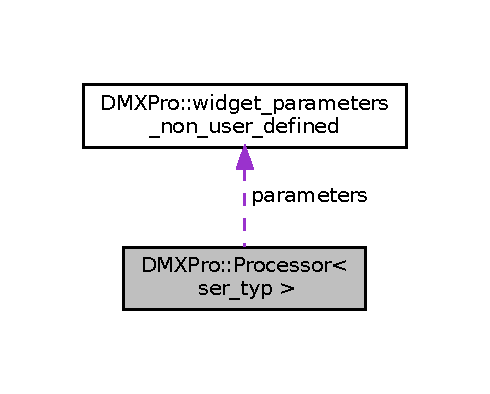
\includegraphics[width=235pt]{classDMXPro_1_1Processor__coll__graph}
\end{center}
\end{figure}
\subsection*{Public Member Functions}
\begin{DoxyCompactItemize}
\item 
\hyperlink{classDMXPro_1_1Processor_a1fc149f6c2f24a8fb8e2562c253e0ddf}{Processor} (ser\+\_\+typ \&ser\+\_\+obj, uint32\+\_\+t serial, uint8\+\_\+t $\ast$data, uint16\+\_\+t max\+\_\+channels)
\item 
\hyperlink{namespaceDMXPro_a0b4335b3ed2abbd803e6d33c54d6ac6d}{Event} \hyperlink{classDMXPro_1_1Processor_a3391d1ac0d213bdadbed8313d15584d6}{process} (void)
\begin{DoxyCompactList}\small\item\em Processes the incoming packet stream from the Host PC and returns events based on the processed packets. \end{DoxyCompactList}\item 
uint8\+\_\+t \hyperlink{classDMXPro_1_1Processor_a93e71e87740b0464504f829297bb654f}{operator\mbox{[}$\,$\mbox{]}} (uint16\+\_\+t c)
\begin{DoxyCompactList}\small\item\em Obtains the D\+MX data value for a particular D\+MX channel. \end{DoxyCompactList}\item 
void \hyperlink{classDMXPro_1_1Processor_ae65b0e05885eb2878544e5bedcded36c}{upload\+\_\+dmx} (bool valid, const uint8\+\_\+t $\ast$data, uint16\+\_\+t length)
\begin{DoxyCompactList}\small\item\em Sends dmx data to the host PC, via the provided communication channel. \end{DoxyCompactList}\end{DoxyCompactItemize}
\subsection*{Private Types}
\begin{DoxyCompactItemize}
\item 
enum \hyperlink{classDMXPro_1_1Processor_ab5c1e3e1ccd6dd60b9e05c3438341a24}{States} \{ \newline
\hyperlink{classDMXPro_1_1Processor_ab5c1e3e1ccd6dd60b9e05c3438341a24a334c4a4c42fdb79d7ebc3e73b517e6f8}{States\+::none}, 
\hyperlink{classDMXPro_1_1Processor_ab5c1e3e1ccd6dd60b9e05c3438341a24aa166b18047c9a32d2a648dfa1b753363}{States\+::type\+\_\+wait}, 
\hyperlink{classDMXPro_1_1Processor_ab5c1e3e1ccd6dd60b9e05c3438341a24aeaa16feeea9709ce06294b39d7bb4d50}{States\+::length\+\_\+wait}, 
\hyperlink{classDMXPro_1_1Processor_ab5c1e3e1ccd6dd60b9e05c3438341a24acddf62aa8552e8b51ec4d46fd1c47f04}{States\+::data\+\_\+wait}, 
\newline
\hyperlink{classDMXPro_1_1Processor_ab5c1e3e1ccd6dd60b9e05c3438341a24a49d6255a7efb5d93ffcc2f7bbb7a5180}{States\+::end\+\_\+wait}
 \}
\end{DoxyCompactItemize}
\subsection*{Private Member Functions}
\begin{DoxyCompactItemize}
\item 
void \hyperlink{classDMXPro_1_1Processor_a3632542df4aae7719d6ab2e964271e36}{set\+\_\+channel} (uint16\+\_\+t channel\+\_\+number, uint8\+\_\+t value)
\begin{DoxyCompactList}\small\item\em Sets a D\+MX channel to a certain value. \end{DoxyCompactList}\item 
void \hyperlink{classDMXPro_1_1Processor_a792bcffc8ca31367baf568305516dac8}{obtain\+\_\+start\+\_\+byte} ()
\begin{DoxyCompactList}\small\item\em \hyperlink{classDMXPro_1_1Processor}{Processor} state machine function. Checks that the next incoming byte is indeed the start byte. \end{DoxyCompactList}\item 
void \hyperlink{classDMXPro_1_1Processor_ad2e73b51c77d95ff948b2b994eba3cfd}{obtain\+\_\+type\+\_\+byte} ()
\begin{DoxyCompactList}\small\item\em \hyperlink{classDMXPro_1_1Processor}{Processor} state machine function. Stores the next incoming value as the type byte. \end{DoxyCompactList}\item 
void \hyperlink{classDMXPro_1_1Processor_a229f4d96176b4fbcda52fa09e44e297a}{obtain\+\_\+length\+\_\+bytes} ()
\begin{DoxyCompactList}\small\item\em \hyperlink{classDMXPro_1_1Processor}{Processor} state machine function. Reads in the next two length bytes, and checks that the resulting length value derived from those two bytes is valid. \end{DoxyCompactList}\item 
bool \hyperlink{classDMXPro_1_1Processor_ad8895162387072e0c5c44101f516b351}{obtain\+\_\+end\+\_\+byte} ()
\begin{DoxyCompactList}\small\item\em \hyperlink{classDMXPro_1_1Processor}{Processor} state machine function. Checks that the next incoming byte is indeed the end delimiter byte. \end{DoxyCompactList}\item 
void \hyperlink{classDMXPro_1_1Processor_a21649894efa9a8e88148b5832b15e4b0}{discard\+\_\+data\+\_\+segment} ()
\begin{DoxyCompactList}\small\item\em One of the actions taken when the state machine is tasked to obtain the payload data. This function represents the action to discard the payload data. (Run for message types that are not supported, or not implemented, where the data does not concern us) \end{DoxyCompactList}\item 
void \hyperlink{classDMXPro_1_1Processor_a30fe8b5251a30f8662dbb6d312c4fe25}{store\+\_\+widget\+\_\+parameters\+\_\+acq\+\_\+data} ()
\item 
void \hyperlink{classDMXPro_1_1Processor_aa2e16c41e09b7823570132f02d57ba34}{get\+\_\+widget\+\_\+parameters\+\_\+acq\+\_\+data} ()
\item 
void \hyperlink{classDMXPro_1_1Processor_a27f23f48cc4fe881915e813a972eb43b}{send\+\_\+dmx\+\_\+data\+\_\+acq\+\_\+data} ()
\item 
void \hyperlink{classDMXPro_1_1Processor_a1170e4aae92ed4bf740020e13602e648}{obtain\+\_\+data\+\_\+bytes} ()
\item 
void \hyperlink{classDMXPro_1_1Processor_a554484560a2dcc0d5763074a584074bb}{send\+\_\+data} (uint8\+\_\+t $\ast$data, \hyperlink{namespaceDMXPro_a001319de95203723f1bd253fec3186cd}{labels} label, uint16\+\_\+t data\+\_\+size, uint16\+\_\+t append\+\_\+zeroes)
\item 
\hyperlink{namespaceDMXPro_a0b4335b3ed2abbd803e6d33c54d6ac6d}{Event} \hyperlink{classDMXPro_1_1Processor_a21c28c13ee050cabdaabc6d869137dcc}{process\+\_\+message} ()
\end{DoxyCompactItemize}
\subsection*{Private Attributes}
\begin{DoxyCompactItemize}
\item 
\hyperlink{classDMXPro_1_1Processor_ab5c1e3e1ccd6dd60b9e05c3438341a24}{States} \hyperlink{classDMXPro_1_1Processor_a1b0ea97d2f76042a9c5c65d6fbb88df0}{state} =\hyperlink{classDMXPro_1_1Processor_ab5c1e3e1ccd6dd60b9e05c3438341a24a334c4a4c42fdb79d7ebc3e73b517e6f8}{States\+::none}
\item 
\hyperlink{namespaceDMXPro_a001319de95203723f1bd253fec3186cd}{labels} \hyperlink{classDMXPro_1_1Processor_a7cda5025516aa2cdf2fdab4928652678}{message\+\_\+label}
\item 
uint16\+\_\+t \hyperlink{classDMXPro_1_1Processor_a240aa5037cd16241045aa59cf7778924}{message\+\_\+data\+\_\+length}
\item 
uint16\+\_\+t \hyperlink{classDMXPro_1_1Processor_a1ac91fd49f9650bc45ee1a1ad8e5f39f}{message\+\_\+data\+\_\+received}
\item 
uint8\+\_\+t $\ast$ \hyperlink{classDMXPro_1_1Processor_a0dc6a66e64a393c6ca41f0d596edca3b}{dmx\+\_\+data}
\item 
uint16\+\_\+t \hyperlink{classDMXPro_1_1Processor_a1286b3edd8b9eea1c27853ac48c3845f}{dmx\+\_\+max\+\_\+channels}
\item 
\hyperlink{structDMXPro_1_1widget__parameters__non__user__defined}{widget\+\_\+parameters\+\_\+non\+\_\+user\+\_\+defined} \hyperlink{classDMXPro_1_1Processor_ab862c9d44d1abdcd029d0d47da7e928d}{parameters}
\item 
uint16\+\_\+t \hyperlink{classDMXPro_1_1Processor_a45fb005d1d5aa98896a8a29362f5a7e8}{widget\+\_\+user\+\_\+configuration\+\_\+size} =0
\item 
ser\+\_\+typ $\ast$ \hyperlink{classDMXPro_1_1Processor_afad2bc7129dfc3e1f039af5ae0243802}{ser}
\item 
uint32\+\_\+t \hyperlink{classDMXPro_1_1Processor_ab3573fe1aa615ec51dfd826c7f2747f9}{serial\+\_\+number}
\end{DoxyCompactItemize}


\subsection{Member Enumeration Documentation}
\mbox{\Hypertarget{classDMXPro_1_1Processor_ab5c1e3e1ccd6dd60b9e05c3438341a24}\label{classDMXPro_1_1Processor_ab5c1e3e1ccd6dd60b9e05c3438341a24}} 
\index{D\+M\+X\+Pro\+::\+Processor@{D\+M\+X\+Pro\+::\+Processor}!States@{States}}
\index{States@{States}!D\+M\+X\+Pro\+::\+Processor@{D\+M\+X\+Pro\+::\+Processor}}
\subsubsection{\texorpdfstring{States}{States}}
{\footnotesize\ttfamily template$<$typename ser\+\_\+typ $>$ \\
enum \hyperlink{classDMXPro_1_1Processor_ab5c1e3e1ccd6dd60b9e05c3438341a24}{D\+M\+X\+Pro\+::\+Processor\+::\+States}\hspace{0.3cm}{\ttfamily [strong]}, {\ttfamily [private]}}

\begin{DoxyEnumFields}{Enumerator}
\raisebox{\heightof{T}}[0pt][0pt]{\index{none@{none}!D\+M\+X\+Pro\+::\+Processor@{D\+M\+X\+Pro\+::\+Processor}}\index{D\+M\+X\+Pro\+::\+Processor@{D\+M\+X\+Pro\+::\+Processor}!none@{none}}}\mbox{\Hypertarget{classDMXPro_1_1Processor_ab5c1e3e1ccd6dd60b9e05c3438341a24a334c4a4c42fdb79d7ebc3e73b517e6f8}\label{classDMXPro_1_1Processor_ab5c1e3e1ccd6dd60b9e05c3438341a24a334c4a4c42fdb79d7ebc3e73b517e6f8}} 
none&No message being processed \\
\hline

\raisebox{\heightof{T}}[0pt][0pt]{\index{type\+\_\+wait@{type\+\_\+wait}!D\+M\+X\+Pro\+::\+Processor@{D\+M\+X\+Pro\+::\+Processor}}\index{D\+M\+X\+Pro\+::\+Processor@{D\+M\+X\+Pro\+::\+Processor}!type\+\_\+wait@{type\+\_\+wait}}}\mbox{\Hypertarget{classDMXPro_1_1Processor_ab5c1e3e1ccd6dd60b9e05c3438341a24aa166b18047c9a32d2a648dfa1b753363}\label{classDMXPro_1_1Processor_ab5c1e3e1ccd6dd60b9e05c3438341a24aa166b18047c9a32d2a648dfa1b753363}} 
type\+\_\+wait&Waiting for message type \\
\hline

\raisebox{\heightof{T}}[0pt][0pt]{\index{length\+\_\+wait@{length\+\_\+wait}!D\+M\+X\+Pro\+::\+Processor@{D\+M\+X\+Pro\+::\+Processor}}\index{D\+M\+X\+Pro\+::\+Processor@{D\+M\+X\+Pro\+::\+Processor}!length\+\_\+wait@{length\+\_\+wait}}}\mbox{\Hypertarget{classDMXPro_1_1Processor_ab5c1e3e1ccd6dd60b9e05c3438341a24aeaa16feeea9709ce06294b39d7bb4d50}\label{classDMXPro_1_1Processor_ab5c1e3e1ccd6dd60b9e05c3438341a24aeaa16feeea9709ce06294b39d7bb4d50}} 
length\+\_\+wait&Waiting for length \\
\hline

\raisebox{\heightof{T}}[0pt][0pt]{\index{data\+\_\+wait@{data\+\_\+wait}!D\+M\+X\+Pro\+::\+Processor@{D\+M\+X\+Pro\+::\+Processor}}\index{D\+M\+X\+Pro\+::\+Processor@{D\+M\+X\+Pro\+::\+Processor}!data\+\_\+wait@{data\+\_\+wait}}}\mbox{\Hypertarget{classDMXPro_1_1Processor_ab5c1e3e1ccd6dd60b9e05c3438341a24acddf62aa8552e8b51ec4d46fd1c47f04}\label{classDMXPro_1_1Processor_ab5c1e3e1ccd6dd60b9e05c3438341a24acddf62aa8552e8b51ec4d46fd1c47f04}} 
data\+\_\+wait&Waiting for data \\
\hline

\raisebox{\heightof{T}}[0pt][0pt]{\index{end\+\_\+wait@{end\+\_\+wait}!D\+M\+X\+Pro\+::\+Processor@{D\+M\+X\+Pro\+::\+Processor}}\index{D\+M\+X\+Pro\+::\+Processor@{D\+M\+X\+Pro\+::\+Processor}!end\+\_\+wait@{end\+\_\+wait}}}\mbox{\Hypertarget{classDMXPro_1_1Processor_ab5c1e3e1ccd6dd60b9e05c3438341a24a49d6255a7efb5d93ffcc2f7bbb7a5180}\label{classDMXPro_1_1Processor_ab5c1e3e1ccd6dd60b9e05c3438341a24a49d6255a7efb5d93ffcc2f7bbb7a5180}} 
end\+\_\+wait&Waiting for message end \\
\hline

\end{DoxyEnumFields}


\subsection{Constructor \& Destructor Documentation}
\mbox{\Hypertarget{classDMXPro_1_1Processor_a1fc149f6c2f24a8fb8e2562c253e0ddf}\label{classDMXPro_1_1Processor_a1fc149f6c2f24a8fb8e2562c253e0ddf}} 
\index{D\+M\+X\+Pro\+::\+Processor@{D\+M\+X\+Pro\+::\+Processor}!Processor@{Processor}}
\index{Processor@{Processor}!D\+M\+X\+Pro\+::\+Processor@{D\+M\+X\+Pro\+::\+Processor}}
\subsubsection{\texorpdfstring{Processor()}{Processor()}}
{\footnotesize\ttfamily template$<$typename ser\+\_\+typ $>$ \\
\hyperlink{classDMXPro_1_1Processor}{D\+M\+X\+Pro\+::\+Processor}$<$ ser\+\_\+typ $>$\+::\hyperlink{classDMXPro_1_1Processor}{Processor} (\begin{DoxyParamCaption}\item[{ser\+\_\+typ \&}]{ser\+\_\+obj,  }\item[{uint32\+\_\+t}]{serial,  }\item[{uint8\+\_\+t $\ast$}]{data,  }\item[{uint16\+\_\+t}]{max\+\_\+channels }\end{DoxyParamCaption})\hspace{0.3cm}{\ttfamily [inline]}}



\subsection{Member Function Documentation}
\mbox{\Hypertarget{classDMXPro_1_1Processor_a21649894efa9a8e88148b5832b15e4b0}\label{classDMXPro_1_1Processor_a21649894efa9a8e88148b5832b15e4b0}} 
\index{D\+M\+X\+Pro\+::\+Processor@{D\+M\+X\+Pro\+::\+Processor}!discard\+\_\+data\+\_\+segment@{discard\+\_\+data\+\_\+segment}}
\index{discard\+\_\+data\+\_\+segment@{discard\+\_\+data\+\_\+segment}!D\+M\+X\+Pro\+::\+Processor@{D\+M\+X\+Pro\+::\+Processor}}
\subsubsection{\texorpdfstring{discard\+\_\+data\+\_\+segment()}{discard\_data\_segment()}}
{\footnotesize\ttfamily template$<$typename ser\+\_\+typ $>$ \\
void \hyperlink{classDMXPro_1_1Processor}{D\+M\+X\+Pro\+::\+Processor}$<$ ser\+\_\+typ $>$\+::discard\+\_\+data\+\_\+segment (\begin{DoxyParamCaption}{ }\end{DoxyParamCaption})\hspace{0.3cm}{\ttfamily [inline]}, {\ttfamily [private]}}



One of the actions taken when the state machine is tasked to obtain the payload data. This function represents the action to discard the payload data. (Run for message types that are not supported, or not implemented, where the data does not concern us) 

One byte of serial data is read in, and subsequently discarded.

\begin{DoxyNote}{Note}
Increments the message\+\_\+data\+\_\+received variable.
\end{DoxyNote}
Alters one variable of non-\/local scope \mbox{\Hypertarget{classDMXPro_1_1Processor_aa2e16c41e09b7823570132f02d57ba34}\label{classDMXPro_1_1Processor_aa2e16c41e09b7823570132f02d57ba34}} 
\index{D\+M\+X\+Pro\+::\+Processor@{D\+M\+X\+Pro\+::\+Processor}!get\+\_\+widget\+\_\+parameters\+\_\+acq\+\_\+data@{get\+\_\+widget\+\_\+parameters\+\_\+acq\+\_\+data}}
\index{get\+\_\+widget\+\_\+parameters\+\_\+acq\+\_\+data@{get\+\_\+widget\+\_\+parameters\+\_\+acq\+\_\+data}!D\+M\+X\+Pro\+::\+Processor@{D\+M\+X\+Pro\+::\+Processor}}
\subsubsection{\texorpdfstring{get\+\_\+widget\+\_\+parameters\+\_\+acq\+\_\+data()}{get\_widget\_parameters\_acq\_data()}}
{\footnotesize\ttfamily template$<$typename ser\+\_\+typ $>$ \\
void \hyperlink{classDMXPro_1_1Processor}{D\+M\+X\+Pro\+::\+Processor}$<$ ser\+\_\+typ $>$\+::get\+\_\+widget\+\_\+parameters\+\_\+acq\+\_\+data (\begin{DoxyParamCaption}{ }\end{DoxyParamCaption})\hspace{0.3cm}{\ttfamily [inline]}, {\ttfamily [private]}}

\mbox{\Hypertarget{classDMXPro_1_1Processor_a1170e4aae92ed4bf740020e13602e648}\label{classDMXPro_1_1Processor_a1170e4aae92ed4bf740020e13602e648}} 
\index{D\+M\+X\+Pro\+::\+Processor@{D\+M\+X\+Pro\+::\+Processor}!obtain\+\_\+data\+\_\+bytes@{obtain\+\_\+data\+\_\+bytes}}
\index{obtain\+\_\+data\+\_\+bytes@{obtain\+\_\+data\+\_\+bytes}!D\+M\+X\+Pro\+::\+Processor@{D\+M\+X\+Pro\+::\+Processor}}
\subsubsection{\texorpdfstring{obtain\+\_\+data\+\_\+bytes()}{obtain\_data\_bytes()}}
{\footnotesize\ttfamily template$<$typename ser\+\_\+typ $>$ \\
void \hyperlink{classDMXPro_1_1Processor}{D\+M\+X\+Pro\+::\+Processor}$<$ ser\+\_\+typ $>$\+::obtain\+\_\+data\+\_\+bytes (\begin{DoxyParamCaption}{ }\end{DoxyParamCaption})\hspace{0.3cm}{\ttfamily [inline]}, {\ttfamily [private]}}

\mbox{\Hypertarget{classDMXPro_1_1Processor_ad8895162387072e0c5c44101f516b351}\label{classDMXPro_1_1Processor_ad8895162387072e0c5c44101f516b351}} 
\index{D\+M\+X\+Pro\+::\+Processor@{D\+M\+X\+Pro\+::\+Processor}!obtain\+\_\+end\+\_\+byte@{obtain\+\_\+end\+\_\+byte}}
\index{obtain\+\_\+end\+\_\+byte@{obtain\+\_\+end\+\_\+byte}!D\+M\+X\+Pro\+::\+Processor@{D\+M\+X\+Pro\+::\+Processor}}
\subsubsection{\texorpdfstring{obtain\+\_\+end\+\_\+byte()}{obtain\_end\_byte()}}
{\footnotesize\ttfamily template$<$typename ser\+\_\+typ $>$ \\
bool \hyperlink{classDMXPro_1_1Processor}{D\+M\+X\+Pro\+::\+Processor}$<$ ser\+\_\+typ $>$\+::obtain\+\_\+end\+\_\+byte (\begin{DoxyParamCaption}{ }\end{DoxyParamCaption})\hspace{0.3cm}{\ttfamily [inline]}, {\ttfamily [private]}}



\hyperlink{classDMXPro_1_1Processor}{Processor} state machine function. Checks that the next incoming byte is indeed the end delimiter byte. 

No matter the validity of the next incoming byte as a end delimiter byte, the state machine is reset.

\begin{DoxyNote}{Note}
Alters the state of the state machine
\end{DoxyNote}
\begin{DoxyPrecond}{Precondition}
The state machine has already acquired a the payload of the message 
\end{DoxyPrecond}
\begin{DoxyPostcond}{Postcondition}
The state machine is now waiting a start byte again
\end{DoxyPostcond}

\begin{DoxyRetVals}{Return values}
{\em true} & A valid message has been received \\
\hline
{\em false} & A non-\/valid message was received \\
\hline
\end{DoxyRetVals}
\mbox{\Hypertarget{classDMXPro_1_1Processor_a229f4d96176b4fbcda52fa09e44e297a}\label{classDMXPro_1_1Processor_a229f4d96176b4fbcda52fa09e44e297a}} 
\index{D\+M\+X\+Pro\+::\+Processor@{D\+M\+X\+Pro\+::\+Processor}!obtain\+\_\+length\+\_\+bytes@{obtain\+\_\+length\+\_\+bytes}}
\index{obtain\+\_\+length\+\_\+bytes@{obtain\+\_\+length\+\_\+bytes}!D\+M\+X\+Pro\+::\+Processor@{D\+M\+X\+Pro\+::\+Processor}}
\subsubsection{\texorpdfstring{obtain\+\_\+length\+\_\+bytes()}{obtain\_length\_bytes()}}
{\footnotesize\ttfamily template$<$typename ser\+\_\+typ $>$ \\
void \hyperlink{classDMXPro_1_1Processor}{D\+M\+X\+Pro\+::\+Processor}$<$ ser\+\_\+typ $>$\+::obtain\+\_\+length\+\_\+bytes (\begin{DoxyParamCaption}{ }\end{DoxyParamCaption})\hspace{0.3cm}{\ttfamily [inline]}, {\ttfamily [private]}}



\hyperlink{classDMXPro_1_1Processor}{Processor} state machine function. Reads in the next two length bytes, and checks that the resulting length value derived from those two bytes is valid. 

\begin{DoxyNote}{Note}
The message\+\_\+data\+\_\+length variable is also updated with this received length value.
\end{DoxyNote}
If the payload length is not valid, the state machine is reset. Otherwise, the state machine is advanced, such that it is now acquiring the payload of the message.

\begin{DoxyNote}{Note}
Alters the state of the state machine, and updates one variable of non-\/local scope.
\end{DoxyNote}
\begin{DoxyPrecond}{Precondition}
The state machine has already acquired the label byte 
\end{DoxyPrecond}
\begin{DoxyPostcond}{Postcondition}
The state machine is now acquiring the payload of the message 
\end{DoxyPostcond}
\mbox{\Hypertarget{classDMXPro_1_1Processor_a792bcffc8ca31367baf568305516dac8}\label{classDMXPro_1_1Processor_a792bcffc8ca31367baf568305516dac8}} 
\index{D\+M\+X\+Pro\+::\+Processor@{D\+M\+X\+Pro\+::\+Processor}!obtain\+\_\+start\+\_\+byte@{obtain\+\_\+start\+\_\+byte}}
\index{obtain\+\_\+start\+\_\+byte@{obtain\+\_\+start\+\_\+byte}!D\+M\+X\+Pro\+::\+Processor@{D\+M\+X\+Pro\+::\+Processor}}
\subsubsection{\texorpdfstring{obtain\+\_\+start\+\_\+byte()}{obtain\_start\_byte()}}
{\footnotesize\ttfamily template$<$typename ser\+\_\+typ $>$ \\
void \hyperlink{classDMXPro_1_1Processor}{D\+M\+X\+Pro\+::\+Processor}$<$ ser\+\_\+typ $>$\+::obtain\+\_\+start\+\_\+byte (\begin{DoxyParamCaption}{ }\end{DoxyParamCaption})\hspace{0.3cm}{\ttfamily [inline]}, {\ttfamily [private]}}



\hyperlink{classDMXPro_1_1Processor}{Processor} state machine function. Checks that the next incoming byte is indeed the start byte. 

If the next incoming byte is not the start byte, the state machine is reset, such that it waits for a start byte again.

\begin{DoxyNote}{Note}
Alters the state of the state machine
\end{DoxyNote}
\begin{DoxyPrecond}{Precondition}
The state machine has been reset 
\end{DoxyPrecond}
\begin{DoxyPostcond}{Postcondition}
The state machine is now waiting for the type byte (label byte in E\+N\+T\+T\+EC nomenclature) 
\end{DoxyPostcond}
\mbox{\Hypertarget{classDMXPro_1_1Processor_ad2e73b51c77d95ff948b2b994eba3cfd}\label{classDMXPro_1_1Processor_ad2e73b51c77d95ff948b2b994eba3cfd}} 
\index{D\+M\+X\+Pro\+::\+Processor@{D\+M\+X\+Pro\+::\+Processor}!obtain\+\_\+type\+\_\+byte@{obtain\+\_\+type\+\_\+byte}}
\index{obtain\+\_\+type\+\_\+byte@{obtain\+\_\+type\+\_\+byte}!D\+M\+X\+Pro\+::\+Processor@{D\+M\+X\+Pro\+::\+Processor}}
\subsubsection{\texorpdfstring{obtain\+\_\+type\+\_\+byte()}{obtain\_type\_byte()}}
{\footnotesize\ttfamily template$<$typename ser\+\_\+typ $>$ \\
void \hyperlink{classDMXPro_1_1Processor}{D\+M\+X\+Pro\+::\+Processor}$<$ ser\+\_\+typ $>$\+::obtain\+\_\+type\+\_\+byte (\begin{DoxyParamCaption}{ }\end{DoxyParamCaption})\hspace{0.3cm}{\ttfamily [inline]}, {\ttfamily [private]}}



\hyperlink{classDMXPro_1_1Processor}{Processor} state machine function. Stores the next incoming value as the type byte. 

\begin{DoxyNote}{Note}
The message\+\_\+label value is updated with this type byte.
\end{DoxyNote}
Alters the state of the state machine, and updates one variable of non-\/local scope.

\begin{DoxyPrecond}{Precondition}
The state machine has already acquired a start byte 
\end{DoxyPrecond}
\begin{DoxyPostcond}{Postcondition}
The state machine is now waiting for the two length bytes 
\end{DoxyPostcond}
\mbox{\Hypertarget{classDMXPro_1_1Processor_a93e71e87740b0464504f829297bb654f}\label{classDMXPro_1_1Processor_a93e71e87740b0464504f829297bb654f}} 
\index{D\+M\+X\+Pro\+::\+Processor@{D\+M\+X\+Pro\+::\+Processor}!operator\mbox{[}\mbox{]}@{operator[]}}
\index{operator\mbox{[}\mbox{]}@{operator[]}!D\+M\+X\+Pro\+::\+Processor@{D\+M\+X\+Pro\+::\+Processor}}
\subsubsection{\texorpdfstring{operator[]()}{operator[]()}}
{\footnotesize\ttfamily template$<$typename ser\+\_\+typ $>$ \\
uint8\+\_\+t \hyperlink{classDMXPro_1_1Processor}{D\+M\+X\+Pro\+::\+Processor}$<$ ser\+\_\+typ $>$\+::operator\mbox{[}$\,$\mbox{]} (\begin{DoxyParamCaption}\item[{uint16\+\_\+t}]{c }\end{DoxyParamCaption})\hspace{0.3cm}{\ttfamily [inline]}}



Obtains the D\+MX data value for a particular D\+MX channel. 


\begin{DoxyParams}[1]{Parameters}
\mbox{\tt in}  & {\em c} & the D\+MX channel to obtain the D\+MX data value for \\
\hline
\end{DoxyParams}
\begin{DoxyWarning}{Warning}
Bounds checking is not performed. If R\+AM storage has not been reserved for this D\+MX channel\textquotesingle{}s data, then the access may result in a dereference of an invalid pointer. 
\end{DoxyWarning}
\begin{DoxyReturn}{Returns}
D\+MX data value \mbox{[}0,255\mbox{]} for that particular D\+MX channel 
\end{DoxyReturn}
\mbox{\Hypertarget{classDMXPro_1_1Processor_a3391d1ac0d213bdadbed8313d15584d6}\label{classDMXPro_1_1Processor_a3391d1ac0d213bdadbed8313d15584d6}} 
\index{D\+M\+X\+Pro\+::\+Processor@{D\+M\+X\+Pro\+::\+Processor}!process@{process}}
\index{process@{process}!D\+M\+X\+Pro\+::\+Processor@{D\+M\+X\+Pro\+::\+Processor}}
\subsubsection{\texorpdfstring{process()}{process()}}
{\footnotesize\ttfamily template$<$typename ser\+\_\+typ $>$ \\
\hyperlink{namespaceDMXPro_a0b4335b3ed2abbd803e6d33c54d6ac6d}{Event} \hyperlink{classDMXPro_1_1Processor}{D\+M\+X\+Pro\+::\+Processor}$<$ ser\+\_\+typ $>$\+::process (\begin{DoxyParamCaption}\item[{void}]{ }\end{DoxyParamCaption})\hspace{0.3cm}{\ttfamily [inline]}}



Processes the incoming packet stream from the Host PC and returns events based on the processed packets. 

\begin{DoxyWarning}{Warning}
This function must be called regularly in order to prevent a communications buffer overflow, which may result in lost packets. This is because this library does not handle any packet processing in the background. Any packet processing is done synchronously. Users may wish to implement asynchronous functionality themselves. 
\end{DoxyWarning}

\begin{DoxyRetVals}{Return values}
{\em An} & event code representing what the host PC requested \\
\hline
\end{DoxyRetVals}
\begin{DoxySeeAlso}{See also}
\hyperlink{namespaceDMXPro_a0b4335b3ed2abbd803e6d33c54d6ac6d}{D\+M\+X\+Pro\+::\+Event} 
\end{DoxySeeAlso}
\mbox{\Hypertarget{classDMXPro_1_1Processor_a21c28c13ee050cabdaabc6d869137dcc}\label{classDMXPro_1_1Processor_a21c28c13ee050cabdaabc6d869137dcc}} 
\index{D\+M\+X\+Pro\+::\+Processor@{D\+M\+X\+Pro\+::\+Processor}!process\+\_\+message@{process\+\_\+message}}
\index{process\+\_\+message@{process\+\_\+message}!D\+M\+X\+Pro\+::\+Processor@{D\+M\+X\+Pro\+::\+Processor}}
\subsubsection{\texorpdfstring{process\+\_\+message()}{process\_message()}}
{\footnotesize\ttfamily template$<$typename ser\+\_\+typ $>$ \\
\hyperlink{namespaceDMXPro_a0b4335b3ed2abbd803e6d33c54d6ac6d}{Event} \hyperlink{classDMXPro_1_1Processor}{D\+M\+X\+Pro\+::\+Processor}$<$ ser\+\_\+typ $>$\+::process\+\_\+message (\begin{DoxyParamCaption}{ }\end{DoxyParamCaption})\hspace{0.3cm}{\ttfamily [inline]}, {\ttfamily [private]}}

Here is the call graph for this function\+:\nopagebreak
\begin{figure}[H]
\begin{center}
\leavevmode
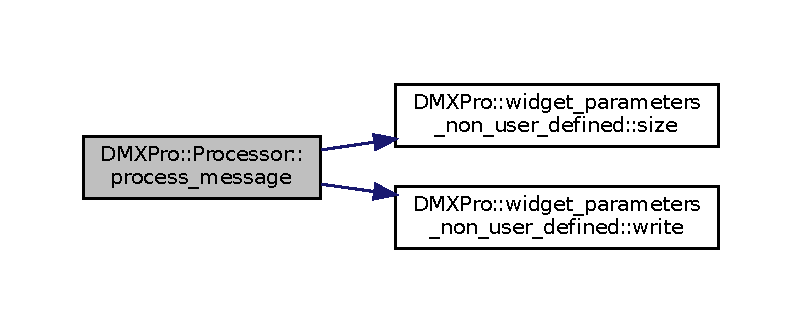
\includegraphics[width=350pt]{classDMXPro_1_1Processor_a21c28c13ee050cabdaabc6d869137dcc_cgraph}
\end{center}
\end{figure}
\mbox{\Hypertarget{classDMXPro_1_1Processor_a554484560a2dcc0d5763074a584074bb}\label{classDMXPro_1_1Processor_a554484560a2dcc0d5763074a584074bb}} 
\index{D\+M\+X\+Pro\+::\+Processor@{D\+M\+X\+Pro\+::\+Processor}!send\+\_\+data@{send\+\_\+data}}
\index{send\+\_\+data@{send\+\_\+data}!D\+M\+X\+Pro\+::\+Processor@{D\+M\+X\+Pro\+::\+Processor}}
\subsubsection{\texorpdfstring{send\+\_\+data()}{send\_data()}}
{\footnotesize\ttfamily template$<$typename ser\+\_\+typ $>$ \\
void \hyperlink{classDMXPro_1_1Processor}{D\+M\+X\+Pro\+::\+Processor}$<$ ser\+\_\+typ $>$\+::send\+\_\+data (\begin{DoxyParamCaption}\item[{uint8\+\_\+t $\ast$}]{data,  }\item[{\hyperlink{namespaceDMXPro_a001319de95203723f1bd253fec3186cd}{labels}}]{label,  }\item[{uint16\+\_\+t}]{data\+\_\+size,  }\item[{uint16\+\_\+t}]{append\+\_\+zeroes }\end{DoxyParamCaption})\hspace{0.3cm}{\ttfamily [inline]}, {\ttfamily [private]}}

\mbox{\Hypertarget{classDMXPro_1_1Processor_a27f23f48cc4fe881915e813a972eb43b}\label{classDMXPro_1_1Processor_a27f23f48cc4fe881915e813a972eb43b}} 
\index{D\+M\+X\+Pro\+::\+Processor@{D\+M\+X\+Pro\+::\+Processor}!send\+\_\+dmx\+\_\+data\+\_\+acq\+\_\+data@{send\+\_\+dmx\+\_\+data\+\_\+acq\+\_\+data}}
\index{send\+\_\+dmx\+\_\+data\+\_\+acq\+\_\+data@{send\+\_\+dmx\+\_\+data\+\_\+acq\+\_\+data}!D\+M\+X\+Pro\+::\+Processor@{D\+M\+X\+Pro\+::\+Processor}}
\subsubsection{\texorpdfstring{send\+\_\+dmx\+\_\+data\+\_\+acq\+\_\+data()}{send\_dmx\_data\_acq\_data()}}
{\footnotesize\ttfamily template$<$typename ser\+\_\+typ $>$ \\
void \hyperlink{classDMXPro_1_1Processor}{D\+M\+X\+Pro\+::\+Processor}$<$ ser\+\_\+typ $>$\+::send\+\_\+dmx\+\_\+data\+\_\+acq\+\_\+data (\begin{DoxyParamCaption}{ }\end{DoxyParamCaption})\hspace{0.3cm}{\ttfamily [inline]}, {\ttfamily [private]}}

\mbox{\Hypertarget{classDMXPro_1_1Processor_a3632542df4aae7719d6ab2e964271e36}\label{classDMXPro_1_1Processor_a3632542df4aae7719d6ab2e964271e36}} 
\index{D\+M\+X\+Pro\+::\+Processor@{D\+M\+X\+Pro\+::\+Processor}!set\+\_\+channel@{set\+\_\+channel}}
\index{set\+\_\+channel@{set\+\_\+channel}!D\+M\+X\+Pro\+::\+Processor@{D\+M\+X\+Pro\+::\+Processor}}
\subsubsection{\texorpdfstring{set\+\_\+channel()}{set\_channel()}}
{\footnotesize\ttfamily template$<$typename ser\+\_\+typ $>$ \\
void \hyperlink{classDMXPro_1_1Processor}{D\+M\+X\+Pro\+::\+Processor}$<$ ser\+\_\+typ $>$\+::set\+\_\+channel (\begin{DoxyParamCaption}\item[{uint16\+\_\+t}]{channel\+\_\+number,  }\item[{uint8\+\_\+t}]{value }\end{DoxyParamCaption})\hspace{0.3cm}{\ttfamily [inline]}, {\ttfamily [private]}}



Sets a D\+MX channel to a certain value. 


\begin{DoxyParams}[1]{Parameters}
\mbox{\tt in}  & {\em channel\+\_\+number} & the D\+MX channel to set, relative to zero \\
\hline
\mbox{\tt in}  & {\em value} & D\+MX channel data value \\
\hline
\end{DoxyParams}
\begin{DoxyNote}{Note}
Bounds checking is performed. When a request is made to set the D\+MX data value of a channel whose storage is not reserved, the request is ignored, silently. 
\end{DoxyNote}
\mbox{\Hypertarget{classDMXPro_1_1Processor_a30fe8b5251a30f8662dbb6d312c4fe25}\label{classDMXPro_1_1Processor_a30fe8b5251a30f8662dbb6d312c4fe25}} 
\index{D\+M\+X\+Pro\+::\+Processor@{D\+M\+X\+Pro\+::\+Processor}!store\+\_\+widget\+\_\+parameters\+\_\+acq\+\_\+data@{store\+\_\+widget\+\_\+parameters\+\_\+acq\+\_\+data}}
\index{store\+\_\+widget\+\_\+parameters\+\_\+acq\+\_\+data@{store\+\_\+widget\+\_\+parameters\+\_\+acq\+\_\+data}!D\+M\+X\+Pro\+::\+Processor@{D\+M\+X\+Pro\+::\+Processor}}
\subsubsection{\texorpdfstring{store\+\_\+widget\+\_\+parameters\+\_\+acq\+\_\+data()}{store\_widget\_parameters\_acq\_data()}}
{\footnotesize\ttfamily template$<$typename ser\+\_\+typ $>$ \\
void \hyperlink{classDMXPro_1_1Processor}{D\+M\+X\+Pro\+::\+Processor}$<$ ser\+\_\+typ $>$\+::store\+\_\+widget\+\_\+parameters\+\_\+acq\+\_\+data (\begin{DoxyParamCaption}{ }\end{DoxyParamCaption})\hspace{0.3cm}{\ttfamily [inline]}, {\ttfamily [private]}}

Here is the call graph for this function\+:\nopagebreak
\begin{figure}[H]
\begin{center}
\leavevmode
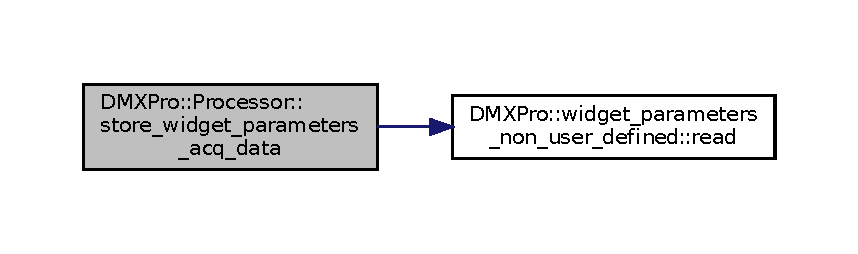
\includegraphics[width=350pt]{classDMXPro_1_1Processor_a30fe8b5251a30f8662dbb6d312c4fe25_cgraph}
\end{center}
\end{figure}
\mbox{\Hypertarget{classDMXPro_1_1Processor_ae65b0e05885eb2878544e5bedcded36c}\label{classDMXPro_1_1Processor_ae65b0e05885eb2878544e5bedcded36c}} 
\index{D\+M\+X\+Pro\+::\+Processor@{D\+M\+X\+Pro\+::\+Processor}!upload\+\_\+dmx@{upload\+\_\+dmx}}
\index{upload\+\_\+dmx@{upload\+\_\+dmx}!D\+M\+X\+Pro\+::\+Processor@{D\+M\+X\+Pro\+::\+Processor}}
\subsubsection{\texorpdfstring{upload\+\_\+dmx()}{upload\_dmx()}}
{\footnotesize\ttfamily template$<$typename ser\+\_\+typ $>$ \\
void \hyperlink{classDMXPro_1_1Processor}{D\+M\+X\+Pro\+::\+Processor}$<$ ser\+\_\+typ $>$\+::upload\+\_\+dmx (\begin{DoxyParamCaption}\item[{bool}]{valid,  }\item[{const uint8\+\_\+t $\ast$}]{data,  }\item[{uint16\+\_\+t}]{length }\end{DoxyParamCaption})\hspace{0.3cm}{\ttfamily [inline]}}



Sends dmx data to the host PC, via the provided communication channel. 


\begin{DoxyParams}{Parameters}
{\em valid} & Set to true to inform PC that dmx data is valid, and we have not dropped incoming D\+MX packets due to processing load. Set to false to indicate that data may be corrupted due to buffer overflow \\
\hline
{\em data} & Pointer to data array containing dmx data to be sent \\
\hline
{\em length} & Length of D\+MX data array (max 512) \\
\hline
\end{DoxyParams}
\begin{DoxyReturn}{Returns}
void 
\end{DoxyReturn}


\subsection{Member Data Documentation}
\mbox{\Hypertarget{classDMXPro_1_1Processor_a0dc6a66e64a393c6ca41f0d596edca3b}\label{classDMXPro_1_1Processor_a0dc6a66e64a393c6ca41f0d596edca3b}} 
\index{D\+M\+X\+Pro\+::\+Processor@{D\+M\+X\+Pro\+::\+Processor}!dmx\+\_\+data@{dmx\+\_\+data}}
\index{dmx\+\_\+data@{dmx\+\_\+data}!D\+M\+X\+Pro\+::\+Processor@{D\+M\+X\+Pro\+::\+Processor}}
\subsubsection{\texorpdfstring{dmx\+\_\+data}{dmx\_data}}
{\footnotesize\ttfamily template$<$typename ser\+\_\+typ $>$ \\
uint8\+\_\+t$\ast$ \hyperlink{classDMXPro_1_1Processor}{D\+M\+X\+Pro\+::\+Processor}$<$ ser\+\_\+typ $>$\+::dmx\+\_\+data\hspace{0.3cm}{\ttfamily [private]}}

D\+MX buffer data location \mbox{\Hypertarget{classDMXPro_1_1Processor_a1286b3edd8b9eea1c27853ac48c3845f}\label{classDMXPro_1_1Processor_a1286b3edd8b9eea1c27853ac48c3845f}} 
\index{D\+M\+X\+Pro\+::\+Processor@{D\+M\+X\+Pro\+::\+Processor}!dmx\+\_\+max\+\_\+channels@{dmx\+\_\+max\+\_\+channels}}
\index{dmx\+\_\+max\+\_\+channels@{dmx\+\_\+max\+\_\+channels}!D\+M\+X\+Pro\+::\+Processor@{D\+M\+X\+Pro\+::\+Processor}}
\subsubsection{\texorpdfstring{dmx\+\_\+max\+\_\+channels}{dmx\_max\_channels}}
{\footnotesize\ttfamily template$<$typename ser\+\_\+typ $>$ \\
uint16\+\_\+t \hyperlink{classDMXPro_1_1Processor}{D\+M\+X\+Pro\+::\+Processor}$<$ ser\+\_\+typ $>$\+::dmx\+\_\+max\+\_\+channels\hspace{0.3cm}{\ttfamily [private]}}

Maximum number of D\+MX channels \mbox{\Hypertarget{classDMXPro_1_1Processor_a240aa5037cd16241045aa59cf7778924}\label{classDMXPro_1_1Processor_a240aa5037cd16241045aa59cf7778924}} 
\index{D\+M\+X\+Pro\+::\+Processor@{D\+M\+X\+Pro\+::\+Processor}!message\+\_\+data\+\_\+length@{message\+\_\+data\+\_\+length}}
\index{message\+\_\+data\+\_\+length@{message\+\_\+data\+\_\+length}!D\+M\+X\+Pro\+::\+Processor@{D\+M\+X\+Pro\+::\+Processor}}
\subsubsection{\texorpdfstring{message\+\_\+data\+\_\+length}{message\_data\_length}}
{\footnotesize\ttfamily template$<$typename ser\+\_\+typ $>$ \\
uint16\+\_\+t \hyperlink{classDMXPro_1_1Processor}{D\+M\+X\+Pro\+::\+Processor}$<$ ser\+\_\+typ $>$\+::message\+\_\+data\+\_\+length\hspace{0.3cm}{\ttfamily [private]}}

Length of message data being processed \mbox{\Hypertarget{classDMXPro_1_1Processor_a1ac91fd49f9650bc45ee1a1ad8e5f39f}\label{classDMXPro_1_1Processor_a1ac91fd49f9650bc45ee1a1ad8e5f39f}} 
\index{D\+M\+X\+Pro\+::\+Processor@{D\+M\+X\+Pro\+::\+Processor}!message\+\_\+data\+\_\+received@{message\+\_\+data\+\_\+received}}
\index{message\+\_\+data\+\_\+received@{message\+\_\+data\+\_\+received}!D\+M\+X\+Pro\+::\+Processor@{D\+M\+X\+Pro\+::\+Processor}}
\subsubsection{\texorpdfstring{message\+\_\+data\+\_\+received}{message\_data\_received}}
{\footnotesize\ttfamily template$<$typename ser\+\_\+typ $>$ \\
uint16\+\_\+t \hyperlink{classDMXPro_1_1Processor}{D\+M\+X\+Pro\+::\+Processor}$<$ ser\+\_\+typ $>$\+::message\+\_\+data\+\_\+received\hspace{0.3cm}{\ttfamily [private]}}

Length of message data that has been received \mbox{\Hypertarget{classDMXPro_1_1Processor_a7cda5025516aa2cdf2fdab4928652678}\label{classDMXPro_1_1Processor_a7cda5025516aa2cdf2fdab4928652678}} 
\index{D\+M\+X\+Pro\+::\+Processor@{D\+M\+X\+Pro\+::\+Processor}!message\+\_\+label@{message\+\_\+label}}
\index{message\+\_\+label@{message\+\_\+label}!D\+M\+X\+Pro\+::\+Processor@{D\+M\+X\+Pro\+::\+Processor}}
\subsubsection{\texorpdfstring{message\+\_\+label}{message\_label}}
{\footnotesize\ttfamily template$<$typename ser\+\_\+typ $>$ \\
\hyperlink{namespaceDMXPro_a001319de95203723f1bd253fec3186cd}{labels} \hyperlink{classDMXPro_1_1Processor}{D\+M\+X\+Pro\+::\+Processor}$<$ ser\+\_\+typ $>$\+::message\+\_\+label\hspace{0.3cm}{\ttfamily [private]}}

Label of message being processed \mbox{\Hypertarget{classDMXPro_1_1Processor_ab862c9d44d1abdcd029d0d47da7e928d}\label{classDMXPro_1_1Processor_ab862c9d44d1abdcd029d0d47da7e928d}} 
\index{D\+M\+X\+Pro\+::\+Processor@{D\+M\+X\+Pro\+::\+Processor}!parameters@{parameters}}
\index{parameters@{parameters}!D\+M\+X\+Pro\+::\+Processor@{D\+M\+X\+Pro\+::\+Processor}}
\subsubsection{\texorpdfstring{parameters}{parameters}}
{\footnotesize\ttfamily template$<$typename ser\+\_\+typ $>$ \\
\hyperlink{structDMXPro_1_1widget__parameters__non__user__defined}{widget\+\_\+parameters\+\_\+non\+\_\+user\+\_\+defined} \hyperlink{classDMXPro_1_1Processor}{D\+M\+X\+Pro\+::\+Processor}$<$ ser\+\_\+typ $>$\+::parameters\hspace{0.3cm}{\ttfamily [private]}}

D\+MX widget parameters \mbox{\Hypertarget{classDMXPro_1_1Processor_afad2bc7129dfc3e1f039af5ae0243802}\label{classDMXPro_1_1Processor_afad2bc7129dfc3e1f039af5ae0243802}} 
\index{D\+M\+X\+Pro\+::\+Processor@{D\+M\+X\+Pro\+::\+Processor}!ser@{ser}}
\index{ser@{ser}!D\+M\+X\+Pro\+::\+Processor@{D\+M\+X\+Pro\+::\+Processor}}
\subsubsection{\texorpdfstring{ser}{ser}}
{\footnotesize\ttfamily template$<$typename ser\+\_\+typ $>$ \\
ser\+\_\+typ$\ast$ \hyperlink{classDMXPro_1_1Processor}{D\+M\+X\+Pro\+::\+Processor}$<$ ser\+\_\+typ $>$\+::ser\hspace{0.3cm}{\ttfamily [private]}}

Pointer to a serial object used to communicate with the PC \mbox{\Hypertarget{classDMXPro_1_1Processor_ab3573fe1aa615ec51dfd826c7f2747f9}\label{classDMXPro_1_1Processor_ab3573fe1aa615ec51dfd826c7f2747f9}} 
\index{D\+M\+X\+Pro\+::\+Processor@{D\+M\+X\+Pro\+::\+Processor}!serial\+\_\+number@{serial\+\_\+number}}
\index{serial\+\_\+number@{serial\+\_\+number}!D\+M\+X\+Pro\+::\+Processor@{D\+M\+X\+Pro\+::\+Processor}}
\subsubsection{\texorpdfstring{serial\+\_\+number}{serial\_number}}
{\footnotesize\ttfamily template$<$typename ser\+\_\+typ $>$ \\
uint32\+\_\+t \hyperlink{classDMXPro_1_1Processor}{D\+M\+X\+Pro\+::\+Processor}$<$ ser\+\_\+typ $>$\+::serial\+\_\+number\hspace{0.3cm}{\ttfamily [private]}}

Widget serial number \mbox{\Hypertarget{classDMXPro_1_1Processor_a1b0ea97d2f76042a9c5c65d6fbb88df0}\label{classDMXPro_1_1Processor_a1b0ea97d2f76042a9c5c65d6fbb88df0}} 
\index{D\+M\+X\+Pro\+::\+Processor@{D\+M\+X\+Pro\+::\+Processor}!state@{state}}
\index{state@{state}!D\+M\+X\+Pro\+::\+Processor@{D\+M\+X\+Pro\+::\+Processor}}
\subsubsection{\texorpdfstring{state}{state}}
{\footnotesize\ttfamily template$<$typename ser\+\_\+typ $>$ \\
\hyperlink{classDMXPro_1_1Processor_ab5c1e3e1ccd6dd60b9e05c3438341a24}{States} \hyperlink{classDMXPro_1_1Processor}{D\+M\+X\+Pro\+::\+Processor}$<$ ser\+\_\+typ $>$\+::state =\hyperlink{classDMXPro_1_1Processor_ab5c1e3e1ccd6dd60b9e05c3438341a24a334c4a4c42fdb79d7ebc3e73b517e6f8}{States\+::none}\hspace{0.3cm}{\ttfamily [private]}}

\hyperlink{classDMXPro_1_1Processor}{Processor} state \mbox{\Hypertarget{classDMXPro_1_1Processor_a45fb005d1d5aa98896a8a29362f5a7e8}\label{classDMXPro_1_1Processor_a45fb005d1d5aa98896a8a29362f5a7e8}} 
\index{D\+M\+X\+Pro\+::\+Processor@{D\+M\+X\+Pro\+::\+Processor}!widget\+\_\+user\+\_\+configuration\+\_\+size@{widget\+\_\+user\+\_\+configuration\+\_\+size}}
\index{widget\+\_\+user\+\_\+configuration\+\_\+size@{widget\+\_\+user\+\_\+configuration\+\_\+size}!D\+M\+X\+Pro\+::\+Processor@{D\+M\+X\+Pro\+::\+Processor}}
\subsubsection{\texorpdfstring{widget\+\_\+user\+\_\+configuration\+\_\+size}{widget\_user\_configuration\_size}}
{\footnotesize\ttfamily template$<$typename ser\+\_\+typ $>$ \\
uint16\+\_\+t \hyperlink{classDMXPro_1_1Processor}{D\+M\+X\+Pro\+::\+Processor}$<$ ser\+\_\+typ $>$\+::widget\+\_\+user\+\_\+configuration\+\_\+size =0\hspace{0.3cm}{\ttfamily [private]}}

Widget user configuration size (Size of the user-\/defined widget configuration array in the packet) 

The documentation for this class was generated from the following file\+:\begin{DoxyCompactItemize}
\item 
src/\hyperlink{arduino__DMXPro_8h}{arduino\+\_\+\+D\+M\+X\+Pro.\+h}\end{DoxyCompactItemize}

\hypertarget{structDMXPro_1_1widget__parameters__non__user__defined}{}\section{D\+M\+X\+Pro\+:\+:widget\+\_\+parameters\+\_\+non\+\_\+user\+\_\+defined Struct Reference}
\label{structDMXPro_1_1widget__parameters__non__user__defined}\index{D\+M\+X\+Pro\+::widget\+\_\+parameters\+\_\+non\+\_\+user\+\_\+defined@{D\+M\+X\+Pro\+::widget\+\_\+parameters\+\_\+non\+\_\+user\+\_\+defined}}


Structure representing widget parameters that are not defined arbitrarily.  




{\ttfamily \#include $<$arduino\+\_\+\+D\+M\+X\+Pro.\+h$>$}

\subsection*{Public Member Functions}
\begin{DoxyCompactItemize}
\item 
void \hyperlink{structDMXPro_1_1widget__parameters__non__user__defined_a25c093468533097e9b06f395b98381e4}{write} (uint8\+\_\+t $\ast$target)
\item 
void \hyperlink{structDMXPro_1_1widget__parameters__non__user__defined_a90e515d288e7fc8582622bc3719774ec}{read} (uint8\+\_\+t $\ast$source)
\end{DoxyCompactItemize}
\subsection*{Static Public Member Functions}
\begin{DoxyCompactItemize}
\item 
static constexpr uint8\+\_\+t \hyperlink{structDMXPro_1_1widget__parameters__non__user__defined_a0fe1584a072b9fa8b3f18c3e5b61cedc}{size} ()
\end{DoxyCompactItemize}
\subsection*{Public Attributes}
\begin{DoxyCompactItemize}
\item 
const uint16\+\_\+t \hyperlink{structDMXPro_1_1widget__parameters__non__user__defined_a499e78f749932ed279e0d23a2716f2ae}{firmware\+\_\+version} =0x0100
\item 
uint8\+\_\+t \hyperlink{structDMXPro_1_1widget__parameters__non__user__defined_ae371cdc7a6b668f9360b1e4eee833f5e}{break\+\_\+time} =9
\item 
uint8\+\_\+t \hyperlink{structDMXPro_1_1widget__parameters__non__user__defined_a0622e5c23a87de586955dd8758ec6a2d}{mark\+\_\+after\+\_\+break\+\_\+time} =1
\item 
uint8\+\_\+t \hyperlink{structDMXPro_1_1widget__parameters__non__user__defined_a6e4165490ca2ba56ce3760d6053bb17a}{dmx\+\_\+output\+\_\+rate} =40
\end{DoxyCompactItemize}


\subsection{Detailed Description}
Structure representing widget parameters that are not defined arbitrarily. 

\subsection{Member Function Documentation}
\mbox{\Hypertarget{structDMXPro_1_1widget__parameters__non__user__defined_a90e515d288e7fc8582622bc3719774ec}\label{structDMXPro_1_1widget__parameters__non__user__defined_a90e515d288e7fc8582622bc3719774ec}} 
\index{D\+M\+X\+Pro\+::widget\+\_\+parameters\+\_\+non\+\_\+user\+\_\+defined@{D\+M\+X\+Pro\+::widget\+\_\+parameters\+\_\+non\+\_\+user\+\_\+defined}!read@{read}}
\index{read@{read}!D\+M\+X\+Pro\+::widget\+\_\+parameters\+\_\+non\+\_\+user\+\_\+defined@{D\+M\+X\+Pro\+::widget\+\_\+parameters\+\_\+non\+\_\+user\+\_\+defined}}
\subsubsection{\texorpdfstring{read()}{read()}}
{\footnotesize\ttfamily void D\+M\+X\+Pro\+::widget\+\_\+parameters\+\_\+non\+\_\+user\+\_\+defined\+::read (\begin{DoxyParamCaption}\item[{uint8\+\_\+t $\ast$}]{source }\end{DoxyParamCaption})\hspace{0.3cm}{\ttfamily [inline]}}

\mbox{\Hypertarget{structDMXPro_1_1widget__parameters__non__user__defined_a0fe1584a072b9fa8b3f18c3e5b61cedc}\label{structDMXPro_1_1widget__parameters__non__user__defined_a0fe1584a072b9fa8b3f18c3e5b61cedc}} 
\index{D\+M\+X\+Pro\+::widget\+\_\+parameters\+\_\+non\+\_\+user\+\_\+defined@{D\+M\+X\+Pro\+::widget\+\_\+parameters\+\_\+non\+\_\+user\+\_\+defined}!size@{size}}
\index{size@{size}!D\+M\+X\+Pro\+::widget\+\_\+parameters\+\_\+non\+\_\+user\+\_\+defined@{D\+M\+X\+Pro\+::widget\+\_\+parameters\+\_\+non\+\_\+user\+\_\+defined}}
\subsubsection{\texorpdfstring{size()}{size()}}
{\footnotesize\ttfamily static constexpr uint8\+\_\+t D\+M\+X\+Pro\+::widget\+\_\+parameters\+\_\+non\+\_\+user\+\_\+defined\+::size (\begin{DoxyParamCaption}{ }\end{DoxyParamCaption})\hspace{0.3cm}{\ttfamily [inline]}, {\ttfamily [static]}}

\mbox{\Hypertarget{structDMXPro_1_1widget__parameters__non__user__defined_a25c093468533097e9b06f395b98381e4}\label{structDMXPro_1_1widget__parameters__non__user__defined_a25c093468533097e9b06f395b98381e4}} 
\index{D\+M\+X\+Pro\+::widget\+\_\+parameters\+\_\+non\+\_\+user\+\_\+defined@{D\+M\+X\+Pro\+::widget\+\_\+parameters\+\_\+non\+\_\+user\+\_\+defined}!write@{write}}
\index{write@{write}!D\+M\+X\+Pro\+::widget\+\_\+parameters\+\_\+non\+\_\+user\+\_\+defined@{D\+M\+X\+Pro\+::widget\+\_\+parameters\+\_\+non\+\_\+user\+\_\+defined}}
\subsubsection{\texorpdfstring{write()}{write()}}
{\footnotesize\ttfamily void D\+M\+X\+Pro\+::widget\+\_\+parameters\+\_\+non\+\_\+user\+\_\+defined\+::write (\begin{DoxyParamCaption}\item[{uint8\+\_\+t $\ast$}]{target }\end{DoxyParamCaption})\hspace{0.3cm}{\ttfamily [inline]}}



\subsection{Member Data Documentation}
\mbox{\Hypertarget{structDMXPro_1_1widget__parameters__non__user__defined_ae371cdc7a6b668f9360b1e4eee833f5e}\label{structDMXPro_1_1widget__parameters__non__user__defined_ae371cdc7a6b668f9360b1e4eee833f5e}} 
\index{D\+M\+X\+Pro\+::widget\+\_\+parameters\+\_\+non\+\_\+user\+\_\+defined@{D\+M\+X\+Pro\+::widget\+\_\+parameters\+\_\+non\+\_\+user\+\_\+defined}!break\+\_\+time@{break\+\_\+time}}
\index{break\+\_\+time@{break\+\_\+time}!D\+M\+X\+Pro\+::widget\+\_\+parameters\+\_\+non\+\_\+user\+\_\+defined@{D\+M\+X\+Pro\+::widget\+\_\+parameters\+\_\+non\+\_\+user\+\_\+defined}}
\subsubsection{\texorpdfstring{break\+\_\+time}{break\_time}}
{\footnotesize\ttfamily uint8\+\_\+t D\+M\+X\+Pro\+::widget\+\_\+parameters\+\_\+non\+\_\+user\+\_\+defined\+::break\+\_\+time =9}

D\+MX break time \mbox{\Hypertarget{structDMXPro_1_1widget__parameters__non__user__defined_a6e4165490ca2ba56ce3760d6053bb17a}\label{structDMXPro_1_1widget__parameters__non__user__defined_a6e4165490ca2ba56ce3760d6053bb17a}} 
\index{D\+M\+X\+Pro\+::widget\+\_\+parameters\+\_\+non\+\_\+user\+\_\+defined@{D\+M\+X\+Pro\+::widget\+\_\+parameters\+\_\+non\+\_\+user\+\_\+defined}!dmx\+\_\+output\+\_\+rate@{dmx\+\_\+output\+\_\+rate}}
\index{dmx\+\_\+output\+\_\+rate@{dmx\+\_\+output\+\_\+rate}!D\+M\+X\+Pro\+::widget\+\_\+parameters\+\_\+non\+\_\+user\+\_\+defined@{D\+M\+X\+Pro\+::widget\+\_\+parameters\+\_\+non\+\_\+user\+\_\+defined}}
\subsubsection{\texorpdfstring{dmx\+\_\+output\+\_\+rate}{dmx\_output\_rate}}
{\footnotesize\ttfamily uint8\+\_\+t D\+M\+X\+Pro\+::widget\+\_\+parameters\+\_\+non\+\_\+user\+\_\+defined\+::dmx\+\_\+output\+\_\+rate =40}

D\+MX output rate \mbox{\Hypertarget{structDMXPro_1_1widget__parameters__non__user__defined_a499e78f749932ed279e0d23a2716f2ae}\label{structDMXPro_1_1widget__parameters__non__user__defined_a499e78f749932ed279e0d23a2716f2ae}} 
\index{D\+M\+X\+Pro\+::widget\+\_\+parameters\+\_\+non\+\_\+user\+\_\+defined@{D\+M\+X\+Pro\+::widget\+\_\+parameters\+\_\+non\+\_\+user\+\_\+defined}!firmware\+\_\+version@{firmware\+\_\+version}}
\index{firmware\+\_\+version@{firmware\+\_\+version}!D\+M\+X\+Pro\+::widget\+\_\+parameters\+\_\+non\+\_\+user\+\_\+defined@{D\+M\+X\+Pro\+::widget\+\_\+parameters\+\_\+non\+\_\+user\+\_\+defined}}
\subsubsection{\texorpdfstring{firmware\+\_\+version}{firmware\_version}}
{\footnotesize\ttfamily const uint16\+\_\+t D\+M\+X\+Pro\+::widget\+\_\+parameters\+\_\+non\+\_\+user\+\_\+defined\+::firmware\+\_\+version =0x0100}

Firmware version, defaulted to one \mbox{\Hypertarget{structDMXPro_1_1widget__parameters__non__user__defined_a0622e5c23a87de586955dd8758ec6a2d}\label{structDMXPro_1_1widget__parameters__non__user__defined_a0622e5c23a87de586955dd8758ec6a2d}} 
\index{D\+M\+X\+Pro\+::widget\+\_\+parameters\+\_\+non\+\_\+user\+\_\+defined@{D\+M\+X\+Pro\+::widget\+\_\+parameters\+\_\+non\+\_\+user\+\_\+defined}!mark\+\_\+after\+\_\+break\+\_\+time@{mark\+\_\+after\+\_\+break\+\_\+time}}
\index{mark\+\_\+after\+\_\+break\+\_\+time@{mark\+\_\+after\+\_\+break\+\_\+time}!D\+M\+X\+Pro\+::widget\+\_\+parameters\+\_\+non\+\_\+user\+\_\+defined@{D\+M\+X\+Pro\+::widget\+\_\+parameters\+\_\+non\+\_\+user\+\_\+defined}}
\subsubsection{\texorpdfstring{mark\+\_\+after\+\_\+break\+\_\+time}{mark\_after\_break\_time}}
{\footnotesize\ttfamily uint8\+\_\+t D\+M\+X\+Pro\+::widget\+\_\+parameters\+\_\+non\+\_\+user\+\_\+defined\+::mark\+\_\+after\+\_\+break\+\_\+time =1}

D\+MX mark-\/after-\/break time 

The documentation for this struct was generated from the following file\+:\begin{DoxyCompactItemize}
\item 
src/\hyperlink{arduino__DMXPro_8h}{arduino\+\_\+\+D\+M\+X\+Pro.\+h}\end{DoxyCompactItemize}

\chapter{File Documentation}
\hypertarget{arduino__DMXPro_8h}{}\section{src/arduino\+\_\+\+D\+M\+X\+Pro.h File Reference}
\label{arduino__DMXPro_8h}\index{src/arduino\+\_\+\+D\+M\+X\+Pro.\+h@{src/arduino\+\_\+\+D\+M\+X\+Pro.\+h}}


Header file for the arduino D\+MX Pro Widget Emulation Library.  


{\ttfamily \#include $<$Arduino.\+h$>$}\newline
Include dependency graph for arduino\+\_\+\+D\+M\+X\+Pro.\+h\+:\nopagebreak
\begin{figure}[H]
\begin{center}
\leavevmode
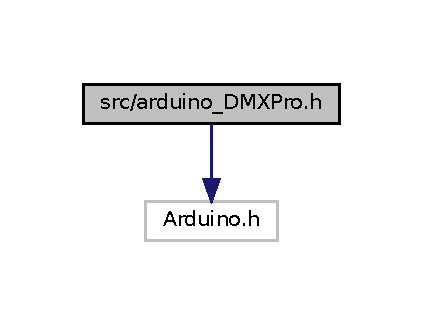
\includegraphics[width=203pt]{arduino__DMXPro_8h__incl}
\end{center}
\end{figure}
\subsection*{Classes}
\begin{DoxyCompactItemize}
\item 
struct \hyperlink{structDMXPro_1_1widget__parameters__non__user__defined}{D\+M\+X\+Pro\+::widget\+\_\+parameters\+\_\+non\+\_\+user\+\_\+defined}
\begin{DoxyCompactList}\small\item\em Structure representing widget parameters that are not defined arbitrarily. \end{DoxyCompactList}\item 
class \hyperlink{classDMXPro_1_1Processor}{D\+M\+X\+Pro\+::\+Processor$<$ ser\+\_\+typ $>$}
\end{DoxyCompactItemize}
\subsection*{Namespaces}
\begin{DoxyCompactItemize}
\item 
 \hyperlink{namespaceDMXPro}{D\+M\+X\+Pro}
\end{DoxyCompactItemize}
\subsection*{Enumerations}
\begin{DoxyCompactItemize}
\item 
enum \hyperlink{namespaceDMXPro_a001319de95203723f1bd253fec3186cd}{D\+M\+X\+Pro\+::labels} \+: uint8\+\_\+t \{ \newline
\hyperlink{namespaceDMXPro_a001319de95203723f1bd253fec3186cda55c46da95be45298c843d4024bd2fee3}{D\+M\+X\+Pro\+::invalid} =0x00, 
\hyperlink{namespaceDMXPro_a001319de95203723f1bd253fec3186cda993f6bf5a5f703a2bb716f14edc559dd}{D\+M\+X\+Pro\+::reprogram\+\_\+firmware} =0x01, 
\hyperlink{namespaceDMXPro_a001319de95203723f1bd253fec3186cdaad9428e105ffc4a4fc6e8f5c1d239f74}{D\+M\+X\+Pro\+::program\+\_\+flash\+\_\+page} =0x02, 
\hyperlink{namespaceDMXPro_a001319de95203723f1bd253fec3186cdaf8caa547d397a97108ca47709f9df577}{D\+M\+X\+Pro\+::program\+\_\+flash\+\_\+page\+\_\+reply} =0x02, 
\newline
\hyperlink{namespaceDMXPro_a001319de95203723f1bd253fec3186cdaeecca4860dc9ba78e33678f4114d4c3c}{D\+M\+X\+Pro\+::get\+\_\+widget\+\_\+parameters} =0x03, 
\hyperlink{namespaceDMXPro_a001319de95203723f1bd253fec3186cdadd2ab9d52b7d9b79893f674ab9c51094}{D\+M\+X\+Pro\+::get\+\_\+widget\+\_\+parameters\+\_\+reply} =0x03, 
\hyperlink{namespaceDMXPro_a001319de95203723f1bd253fec3186cdad29a1d2d4bf0ef748da9ee9be9c6dbac}{D\+M\+X\+Pro\+::store\+\_\+widget\+\_\+parameters} =0x04, 
\hyperlink{namespaceDMXPro_a001319de95203723f1bd253fec3186cda0286e9771de253666cef100914519d76}{D\+M\+X\+Pro\+::receive\+\_\+dmx\+\_\+data} =0x05, 
\newline
\hyperlink{namespaceDMXPro_a001319de95203723f1bd253fec3186cda9b6d6b2db8164ed8608dd614951d381d}{D\+M\+X\+Pro\+::send\+\_\+dmx\+\_\+data} =0x06, 
\hyperlink{namespaceDMXPro_a001319de95203723f1bd253fec3186cda484d7b8788d281d1107e5a24214a8d97}{D\+M\+X\+Pro\+::get\+\_\+widget\+\_\+serial} =0x0a, 
\hyperlink{namespaceDMXPro_a001319de95203723f1bd253fec3186cda2f020af04645c0ec2e64ab77adf46467}{D\+M\+X\+Pro\+::get\+\_\+widget\+\_\+serial\+\_\+reply} =0x0a, 
\hyperlink{namespaceDMXPro_a001319de95203723f1bd253fec3186cda1f1f0f638168f4d91a5b90cd9474927e}{D\+M\+X\+Pro\+::label\+\_\+max}
 \}\begin{DoxyCompactList}\small\item\em Lists of all message types supported by a D\+MX Pro Widget (Firmware Version 1) \end{DoxyCompactList}
\item 
enum \hyperlink{namespaceDMXPro_ae978412ae5d98682f1a8f876434749d6}{D\+M\+X\+Pro\+::delimiters} \+: uint8\+\_\+t \{ \hyperlink{namespaceDMXPro_ae978412ae5d98682f1a8f876434749d6ab31985c0a68286d045c874a0d91d300f}{D\+M\+X\+Pro\+::start} =0x7e, 
\hyperlink{namespaceDMXPro_ae978412ae5d98682f1a8f876434749d6a0011ec6afa29407d423b9ad17a00c6dd}{D\+M\+X\+Pro\+::end} =0xe7
 \}\begin{DoxyCompactList}\small\item\em Message delimiters and their values. \end{DoxyCompactList}
\item 
enum \hyperlink{namespaceDMXPro_a0b4335b3ed2abbd803e6d33c54d6ac6d}{D\+M\+X\+Pro\+::\+Event} \+: uint8\+\_\+t \{ \newline
\hyperlink{namespaceDMXPro_a0b4335b3ed2abbd803e6d33c54d6ac6daa4efa255fbd673aa733c90fd0e2c2ca7}{D\+M\+X\+Pro\+::none}, 
\hyperlink{namespaceDMXPro_a0b4335b3ed2abbd803e6d33c54d6ac6da94e16da01d36dcedc1f2fdacdeba2399}{D\+M\+X\+Pro\+::parameters\+\_\+requested}, 
\hyperlink{namespaceDMXPro_a0b4335b3ed2abbd803e6d33c54d6ac6da013201c7d4dde91ca5c8ce7a2b60e71d}{D\+M\+X\+Pro\+::parameters\+\_\+changed}, 
\hyperlink{namespaceDMXPro_a0b4335b3ed2abbd803e6d33c54d6ac6da2135a293c38559b59c95f8e31c96b2b1}{D\+M\+X\+Pro\+::serial\+\_\+requested}, 
\newline
\hyperlink{namespaceDMXPro_a0b4335b3ed2abbd803e6d33c54d6ac6dad38fe8af23604d427d36da681d413dda}{D\+M\+X\+Pro\+::dmx\+\_\+data}
 \}\begin{DoxyCompactList}\small\item\em Return events from the serial packet processor. \end{DoxyCompactList}
\end{DoxyCompactItemize}


\subsection{Detailed Description}
Header file for the arduino D\+MX Pro Widget Emulation Library. 

\begin{DoxyAuthor}{Author}
Shenghao Yang
\end{DoxyAuthor}
This library only implements Firmware Version 1 (D\+MX Pro, TX only) 
%--- End generated contents ---

% Index
\backmatter
\newpage
\phantomsection
\clearemptydoublepage
\addcontentsline{toc}{chapter}{Index}
\printindex

\end{document}
